%%%%%%%% ICML 2025 EXAMPLE LATEX SUBMISSION FILE %%%%%%%%%%%%%%%%%

\documentclass{article}

% Recommended, but optional, packages for figures and better typesetting:
\usepackage{microtype}
\usepackage{graphicx}
\usepackage{subfigure}
\usepackage{booktabs} % for professional tables
\usepackage{multirow}
\usepackage{tabularx}

% hyperref makes hyperlinks in the resulting PDF.
% If your build breaks (sometimes temporarily if a hyperlink spans a page)
% please comment out the following usepackage line and replace
% \usepackage{icml2025} with \usepackage[nohyperref]{icml2025} above.
\usepackage{hyperref}
\usepackage{tikz}

% Attempt to make hyperref and algorithmic work together better:
\newcommand{\theHalgorithm}{\arabic{algorithm}}

% Use the following line for the initial blind version submitted for review:
 \usepackage[accepted]{icml2025}

% If accepted, instead use the following line for the camera-ready submission:
%\usepackage[accepted]{icml2025}

% For theorems and such
\usepackage{amsmath}
\usepackage{amssymb}
\usepackage{mathtools}
\usepackage{amsthm}
\usepackage{cases}
\usepackage{paralist}

% if you use cleveref..
\usepackage[capitalize,noabbrev]{cleveref}

%%%%%%%%%%%%%%%%%%%%%%%%%%%%%%%%
% THEOREMS
%%%%%%%%%%%%%%%%%%%%%%%%%%%%%%%%
\theoremstyle{plain}
\newtheorem{theorem}{Theorem}[section]
\newtheorem{proposition}[theorem]{Proposition}
\newtheorem{lemma}[theorem]{Lemma}
\newtheorem{corollary}[theorem]{Corollary}
\theoremstyle{definition}
\newtheorem{definition}[theorem]{Definition}
\newtheorem{assumption}[theorem]{Assumption}
\theoremstyle{remark}
\newtheorem{remark}[theorem]{Remark}

% Todonotes is useful during development; simply uncomment the next line
%    and comment out the line below the next line to turn off comments
%\usepackage[disable,textsize=tiny]{todonotes}
\usepackage[textsize=tiny]{todonotes}


% The \icmltitle you define below is probably too long as a header.
% Therefore, a short form for the running title is supplied here:
\icmltitlerunning{Stackelberg Game Preference Optimization for Data-Efficient Alignment of Language Models}

\begin{document}
\onecolumn
% \twocolumn[
\icmltitle{Stackelberg Game Preference Optimization \\ for Data-Efficient Alignment of Language Models}

% It is OKAY to include author information, even for blind
% submissions: the style file will automatically remove it for you
% unless you've provided the [accepted] option to the icml2025
% package.

% List of affiliations: The first argument should be a (short)
% identifier you will use later to specify author affiliations
% Academic affiliations should list Department, University, City, Region, Country
% Industry affiliations should list Company, City, Region, Country

% You can specify symbols, otherwise they are numbered in order.
% Ideally, you should not use this facility. Affiliations will be numbered
% in order of appearance and this is the preferred way.
\icmlsetsymbol{equal}{*}

\begin{icmlauthorlist}
\icmlauthor{Xu Chu}{yyy,sch1}
\icmlauthor{Zhixin Zhang}{sch2,sch1}
\icmlauthor{Tianyu Jia}{zzz,sch1}
\icmlauthor{Yujie Jin}{zzz,sch1}
\end{icmlauthorlist}

\icmlaffiliation{yyy}{Center on Frontiers of Computing Studies, School of Computer Science, Peking University}
\icmlaffiliation{zzz}{School of Computer Science, Peking University}
\icmlaffiliation{sch1}{Key Laboratory of High Confidence Software Technologies, Ministry of Education}
\icmlaffiliation{sch2}{School of Computer Science, Zhejiang University}

\icmlcorrespondingauthor{Xu Chu}{chu\_xu@pku.edu}

% You may provide any keywords that you
% find helpful for describing your paper; these are used to populate
% the "keywords" metadata in the PDF but will not be shown in the document
\icmlkeywords{Machine Learning, ICML}

\vskip 0.3in

% ]
% this must go after the closing bracket ] following \twocolumn[ ...

% This command actually creates the footnote in the first column
% listing the affiliations and the copyright notice.
% The command takes one argument, which is text to display at the start of the footnote.
% The \icmlEqualContribution command is standard text for equal contribution.
% Remove it (just {}) if you do not need this facility.

\printAffiliationsAndNotice{}  % leave blank if no need to mention equal contribution
%\printAffiliationsAndNotice{\icmlEqualContribution} % otherwise use the standard text.

%\begin{abstract}
%Aligning language models with human preferences is critical for real-world deployment, yet existing methods suffer from reliance on a large number of prohibitively costly human annotations. In this paper, we propose \textbf{Stackelberg Game Preference Optimization (SGPO)}, a framework that unifies theoretical guarantees with practical efficiency. Theoretically, we propose SGPO as a two-player Stackelberg game where a policy model (leader) optimizes against worst-case preference distributions generated by an adversarial follower. We prove SGPO converges to a Stackelberg equilibrium with $\mathcal{O}(\epsilon)$-bounded regret under $\epsilon$-bounded annotation noise, in contrast to DPO’s linear regret. Practically, we introduce \textbf{ Stackelberg Self-Annotated Preference Optimization (SSAPO)}, an algorithm that instantiates SGPO with minimal human supervision. Starting with only 1/30 of seed human labels (UltraFeedback), SSAPO iteratively generates synthetic preferences via self-annotation while injecting controlled noise to simulate real-world imperfections. Within \textbf{3 iterations}, SSAPO matches SOTA performance on Alpaca Eval 2.0 with \textbf{30X fewer} human labels.
%\end{abstract}

%\begin{abstract}
%Aligning language models with human preferences is critical for real-world deployment, yet existing methods often rely on prohibitively large amounts of high-quality human annotations. In this paper, we propose \emph{Stackelberg Game Preference Optimization (SGPO)}, a framework that unifies theoretical guarantees with practical efficiency by explicitly modeling alignment as a two-player Stackelberg game. Concretely, a policy model (leader) optimizes against a worst-case preference distribution (follower) within an $\epsilon$-Wasserstein ball, thereby ensuring robustness under moderate annotation noise or distribution shifts.
%Theoretically, we show that SGPO converges to a Stackelberg equilibrium with $\mathcal{O}(\epsilon)$-bounded regret under $\epsilon$-bounded annotation noise. In contrast, Direct Preference Optimization (DPO) can suffer linear regret growth in the size of the distribution mismatch, underscoring SGPO's greater tolerance to labeling errors.
%Practically, we instantiates SGPO with the \emph{Stackelberg Self-Annotated Preference Optimization (SSAPO)} algorithm. Starting with a human labelled seed preference data, SSAPO\footnote{An example code for SSAPO can be found at: \href{https://anonymous.4open.science/r/SSAPO-6818}{anonymous.4open.science/r/SSAPO-6818}} iteratively self-annotates new preferences using the current policy’s rankings and reweights the synthetic preferences adversarially via distributionally robust optimization. Using only 2K seed preference from UltraFeedback dataset, i.e., 1/30 of human labels of the dataset, SSAPO achieves 35.82~\% GPT4 win-rate with Mistral-7B and 40.12\% GPT4 win-rate on Llama3-8B-Instruct with AlpacaEval~2.0 within three round of SSAPO.
%Despite using \emph{30X fewer} human labels, SSAPO can achieve performance on Alpaca Eval~2.0 competitive with state-of-the-art methods within three self-annotation rounds.%Highlighting a scalable path toward label-efficient preference alignment under realistic data constraints.
%\end{abstract}

\begin{abstract}
Aligning language models with human preferences is critical for real-world deployment, but existing methods often require large amounts of high-quality human annotations. Aiming at a data-efficient alignment method, we propose \emph{Stackelberg Game Preference Optimization (SGPO)}, a framework that models alignment as a two-player Stackelberg game, where a policy (leader) optimizes against a worst-case preference distribution (follower) within an $\epsilon$-Wasserstein ball, ensuring robustness to (self-)annotation noise and distribution shifts. SGPO guarantees $\mathcal{O}(\epsilon)$-bounded regret, unlike Direct Preference Optimization (DPO), which suffers from linear regret growth in the distribution mismatch. We instantiate SGPO with the \emph{Stackelberg Self-Annotated Preference Optimization (SSAPO)} algorithm, which iteratively self-annotates preferences and adversarially reweights synthetic annotated preferences. Using only 2K seed preferences, from the UltraFeedback dataset, i.e., 1/30 of human labels in the dataset, our method achieves 35.82\% GPT-4 win-rate with Mistral-7B and 40.12\% with Llama3-8B-Instruct within three rounds of SSAPO.    
% \footnote{An example code for SSAPO can be found at: \href{https://anonymous.4open.science/r/SSAPO-6888}{anonymous.4open.science/r/SSAPO-6888}}
\end{abstract}

%\section{Introduction}


\begin{figure}[t]
\centering
\includegraphics[width=0.6\columnwidth]{figures/evaluation_desiderata_V5.pdf}
\vspace{-0.5cm}
\caption{\systemName is a platform for conducting realistic evaluations of code LLMs, collecting human preferences of coding models with real users, real tasks, and in realistic environments, aimed at addressing the limitations of existing evaluations.
}
\label{fig:motivation}
\end{figure}

\begin{figure*}[t]
\centering
\includegraphics[width=\textwidth]{figures/system_design_v2.png}
\caption{We introduce \systemName, a VSCode extension to collect human preferences of code directly in a developer's IDE. \systemName enables developers to use code completions from various models. The system comprises a) the interface in the user's IDE which presents paired completions to users (left), b) a sampling strategy that picks model pairs to reduce latency (right, top), and c) a prompting scheme that allows diverse LLMs to perform code completions with high fidelity.
Users can select between the top completion (green box) using \texttt{tab} or the bottom completion (blue box) using \texttt{shift+tab}.}
\label{fig:overview}
\end{figure*}

As model capabilities improve, large language models (LLMs) are increasingly integrated into user environments and workflows.
For example, software developers code with AI in integrated developer environments (IDEs)~\citep{peng2023impact}, doctors rely on notes generated through ambient listening~\citep{oberst2024science}, and lawyers consider case evidence identified by electronic discovery systems~\citep{yang2024beyond}.
Increasing deployment of models in productivity tools demands evaluation that more closely reflects real-world circumstances~\citep{hutchinson2022evaluation, saxon2024benchmarks, kapoor2024ai}.
While newer benchmarks and live platforms incorporate human feedback to capture real-world usage, they almost exclusively focus on evaluating LLMs in chat conversations~\citep{zheng2023judging,dubois2023alpacafarm,chiang2024chatbot, kirk2024the}.
Model evaluation must move beyond chat-based interactions and into specialized user environments.



 

In this work, we focus on evaluating LLM-based coding assistants. 
Despite the popularity of these tools---millions of developers use Github Copilot~\citep{Copilot}---existing
evaluations of the coding capabilities of new models exhibit multiple limitations (Figure~\ref{fig:motivation}, bottom).
Traditional ML benchmarks evaluate LLM capabilities by measuring how well a model can complete static, interview-style coding tasks~\citep{chen2021evaluating,austin2021program,jain2024livecodebench, white2024livebench} and lack \emph{real users}. 
User studies recruit real users to evaluate the effectiveness of LLMs as coding assistants, but are often limited to simple programming tasks as opposed to \emph{real tasks}~\citep{vaithilingam2022expectation,ross2023programmer, mozannar2024realhumaneval}.
Recent efforts to collect human feedback such as Chatbot Arena~\citep{chiang2024chatbot} are still removed from a \emph{realistic environment}, resulting in users and data that deviate from typical software development processes.
We introduce \systemName to address these limitations (Figure~\ref{fig:motivation}, top), and we describe our three main contributions below.


\textbf{We deploy \systemName in-the-wild to collect human preferences on code.} 
\systemName is a Visual Studio Code extension, collecting preferences directly in a developer's IDE within their actual workflow (Figure~\ref{fig:overview}).
\systemName provides developers with code completions, akin to the type of support provided by Github Copilot~\citep{Copilot}. 
Over the past 3 months, \systemName has served over~\completions suggestions from 10 state-of-the-art LLMs, 
gathering \sampleCount~votes from \userCount~users.
To collect user preferences,
\systemName presents a novel interface that shows users paired code completions from two different LLMs, which are determined based on a sampling strategy that aims to 
mitigate latency while preserving coverage across model comparisons.
Additionally, we devise a prompting scheme that allows a diverse set of models to perform code completions with high fidelity.
See Section~\ref{sec:system} and Section~\ref{sec:deployment} for details about system design and deployment respectively.



\textbf{We construct a leaderboard of user preferences and find notable differences from existing static benchmarks and human preference leaderboards.}
In general, we observe that smaller models seem to overperform in static benchmarks compared to our leaderboard, while performance among larger models is mixed (Section~\ref{sec:leaderboard_calculation}).
We attribute these differences to the fact that \systemName is exposed to users and tasks that differ drastically from code evaluations in the past. 
Our data spans 103 programming languages and 24 natural languages as well as a variety of real-world applications and code structures, while static benchmarks tend to focus on a specific programming and natural language and task (e.g. coding competition problems).
Additionally, while all of \systemName interactions contain code contexts and the majority involve infilling tasks, a much smaller fraction of Chatbot Arena's coding tasks contain code context, with infilling tasks appearing even more rarely. 
We analyze our data in depth in Section~\ref{subsec:comparison}.



\textbf{We derive new insights into user preferences of code by analyzing \systemName's diverse and distinct data distribution.}
We compare user preferences across different stratifications of input data (e.g., common versus rare languages) and observe which affect observed preferences most (Section~\ref{sec:analysis}).
For example, while user preferences stay relatively consistent across various programming languages, they differ drastically between different task categories (e.g. frontend/backend versus algorithm design).
We also observe variations in user preference due to different features related to code structure 
(e.g., context length and completion patterns).
We open-source \systemName and release a curated subset of code contexts.
Altogether, our results highlight the necessity of model evaluation in realistic and domain-specific settings.





%\bibliographystyle{plainnat}
%\begin{thebibliography}{9}

%\bibitem[Christiano et~al.(2017)]{Christiano2017DeepRLHF}
%Paul Christiano, Jan Leike, Tom Brown, et~al.
%\newblock Deep reinforcement learning from human preferences.
%\newblock In \emph{Advances in Neural Information Processing Systems (NeurIPS)}, 2017.

%\bibitem[Rafailov et~al.(2023)]{Rafailov2023DirectPreference}
%R~Rafailov, Mitchell Wortsman, Ludwig Schmidt, et~al.
%\newblock Direct preference optimization: Your language model is secretly a reward model.
%\newblock \emph{arXiv preprint arXiv:2305.17888}, 2023.

%\bibitem[Von Stackelberg(1934)]{VonStackelberg1934Marktform}
%Heinrich Von Stackelberg.
%\newblock \emph{Marktform und Gleichgewicht}.
%\newblock Julius Springer, 1934.

%\bibitem[Basar and Olsder(1999)]{Basar1999DynamicNG}
%Tamer Basar and Geert~Jan Olsder.
%\newblock \emph{Dynamic Noncooperative Game Theory}.
%\newblock SIAM, 1999.

%\bibitem[Villani(2008)]{Villani2008OptimalTW}
%Cédric Villani.
%\newblock \emph{Optimal transport: old and new}.
%\newblock Springer, 2008.

%\end{thebibliography}

\section{Introduction}
\label{sec:intro}
Recent breakthroughs in large language models (LLMs) have made it increasingly crucial to \emph{align} generated text with human preferences for both usability and safety \citep{Ouyang2022Training,Bai2022Training}. Traditional approaches such as Reinforcement Learning from Human Feedback (RLHF) \citep{Christiano2017Deep} and Direct Preference Optimization (DPO) \citep{Rafailov2023Direct} often require \emph{massive} amounts of meticulously curated preference data. Not only is gathering such a dataset expensive and time-consuming, but any mislabeling can propagate through iterative alignment stages \citep{Casper2023Open}, leading to suboptimal or even unsafe model behaviors. This raises a critical challenge: \emph{How can we achieve preference data-efficient alignment of language models while maintaining robustness to annotation noise?}

From the perspective of data efficiency and robustness, existing alignment approaches often suffer from two main issues:\emph{Self-annotation gaps} and \emph{Lack of equilibrium guarantees under noise}. Recent work explores self-annotation \citep{Lee2024Rlaif,Yuan2024Self,Kim2025Spread}, where an LLM generates labels for new prompt--response pairs instead of relying on humans. While this indeed lowers annotation cost, such methods often treat policy updates and preference annotation as disconnected processes. Consequently, once noisy synthetic preferences are generated, there is limited recourse if the LLM’s self-labels embed systematic biases or errors that can corrupt future training \citep{Chowdhury2024Provably}. Some adversarial training approaches \citep{Cheng2023Adversarial,Wu2024Towards} attempt to counter distributional shifts in preference data, but they often lack formal \emph{equilibrium} guarantees and can lead to unstable optimization cycles in practice. Furthermore, these adversarial approaches are not specifically tailored for data-scarce alignment regimes, thus limiting their applicability when human labels are extremely expensive. \emph{We delay a more thorough \textbf{related work} section in the Appendix~\ref{sec:related_supp}}.

To address these issues, we propose \textbf{Stackelberg Game Preference Optimization (SGPO)}, a framework that models alignment as a \emph{two-player} Stackelberg game between: a \emph{policy} (the leader), which aims to satisfy real human preferences, and an \emph{adversarial preference distribution} (the follower), which explores worst-case shifts within a defined Wasserstein ball of radius $\epsilon$. Drawing inspiration from Stackelberg dynamics \citep{Bacsar1998Dynamic} and optimal transport \citep{Villani2009Optimal}, SGPO ensures that the policy optimizes against the worst plausible shifts in preference data. Specifically, under $\epsilon$-bounded shifts (or annotation noise), we prove that the resulting policy’s regret is at most $\mathcal{O}(\epsilon)$ (see Section~\ref{sec:theory}), whereas standard DPO can incur \emph{linear} regret growth with respect to the magnitude of distribution mismatch. Although our analysis uses $\epsilon$-Wasserstein balls as a tractable model of moderate noise or mismatch, it remains relevant for practical alignment scenarios where annotation errors are not unbounded but still matter.

On top of SGPO, we develop the \textbf{Stackelberg Self-Annotated Preference Optimization (SSAPO)} (Section~\ref{sec:ssapo}) algorithm, a procedure aimed at drastically lowering human annotation needs. SSAPO starts with a small human-labeled seed (about $1/30$ of the usual scale in our experiments) and then: \emph{(1) Self-Annotates} newly sampled prompts by generating responses and extracting winner--loser pairs from the current policy's own comparisons. \emph{(2) Adversarially Reweights} these pairs within a Wasserstein ball of radius $\epsilon$, by solving a distributionally robust optimization (DRO) \citep{Esfahani2018Data} program,ensuring that potentially corrupted or unrepresentative synthetic preferences do not overwhelm the policy update.
By iterating these two steps, SSAPO instantiates the SGPO framework, preserving theoretical bounded-regret guarantees while yielding significant data-efficiency gains. In practice, we find that with only 1/30 of the usual human annotations (from the UltraFeedback dataset \citep{Cui2023Ultrafeedback}), SSAPO attains 35.82~\% GPT4 win-rate (24.44\% LC win-rate) on Mistral-7B, 40.12\% win-rate (33.33\% LC win-rate) on Llama3-8B-instruct. Which matches Mixtral Large (21.4\% win-rate and 32.7\% LC win-rate) and Llama3-70B-instruct (33.2\% winrate and 34.4\% LC win-rate) according to the AlphacaEval~2.0 leaderboard~\citep{dubois2024length}.% Concretely, within 3 self-annotation rounds, our model matches methods that use \textbf{30 times} more human-labeled data.

In summary, We formulate DPO-like alignment as a Stackelberg game, demonstrate \emph{existence} of an equilibrium, and establish that \emph{SGPO} achieves an $\mathcal{O}(\epsilon)$ regret bound under $\epsilon$-bounded noise, in contrast to the linear regret behavior of DPO when facing similarly scaled shifts.(Section~\ref{sec:theory}). We implement SGPO via \emph{SSAPO}, which combines self-annotation with distributionaly robust optimization.(Section~\ref{sec:ssapo}) %We tackle the concavity requirement of Standard DRO with piecewise-linear \emph{concave} envelope. We handle large-scale preference data via a \emph{uniform grouping} strategy for parallel subproblem solutions.  
 Extensive experiments show that SSAPO attains strong alignment performance with substantially fewer human labels, thereby showing its real-world viability for cost-effective preference alignment of LLMs (Section~\ref{sec:experiments}).

%Overall, our main contributions are: (1) \textbf{Theoretical Foundation} (Section~\ref{sec:theory}): We formulate alignment under limited labels as a Stackelberg game, demonstrate \emph{existence} of an equilibrium, and establish that \emph{SGPO} achieves an $\mathcal{O}(\epsilon)$ regret bound under $\epsilon$-bounded noise. This stands in contrast to the linear regret behavior of DPO when facing similarly scaled shifts.(Theorems~\ref{thm:existence_se}--\ref{thm:sgpo_regret}). (2) \textbf{Scalable Algorithm} (Section~\ref{sec:ssapo}):  We implement SGPO via \emph{SSAPO}, which combines self-annotation with distributionaly robust optimization (DRO). We tackle the concavity requirement of Standard DRO with piecewise-linear \emph{concave} envelope. We handle large-scale preference data via a \emph{uniform grouping} strategy for parallel subproblem solutions. (3) \textbf{Empirical Validation} (Section~\ref{sec:experiments}): Extensive experiments show that SSAPO attains strong alignment performance with substantially fewer human labels, thereby showing its real-world viability for cost-effective preference alignment of LLMs.
%By furnishing both formal guarantees and an effective, scalable method, we hope to advance the practice of LLM alignment under realistic labeling budgets.

%\section{Related Work}
The landscape of large language model vulnerabilities has been extensively studied in recent literature \cite{crothers2023machinegeneratedtextcomprehensive,shayegani2023surveyvulnerabilitieslargelanguage,Yao_2024,Huang2023ASO}, that propose detailed taxonomies of threats. These works categorize LLM attacks into distinct types, such as adversarial attacks, data poisoning, and specific vulnerabilities related to prompt engineering. Among these, prompt injection attacks have emerged as a significant and distinct category, underscoring their relevance to LLM security.

The following high-level overview of the collected taxonomy of LLM vulnerabilities is defined in \cite{Yao_2024}:
\begin{itemize}
    \item Adversarial Attacks: Data Poisoning, Backdoor Attacks
    \item Inference Attacks: Attribute Inference, Membership Inferences
    \item Extraction Attacks
    \item Bias and Unfairness
Exploitation
    \item Instruction Tuning Attacks: Jailbreaking, Prompt Injection.
\end{itemize}
Prompt injection attacks are further classified in \cite{shayegani2023surveyvulnerabilitieslargelanguage} into the following: Goal hijacking and \textbf{Prompt leakage}.

The reviewed taxonomies underscore the need for comprehensive frameworks to evaluate LLM security. The agentic approach introduced in this paper builds on these insights, automating adversarial testing to address a wide range of scenarios, including those involving prompt leakage and role-specific vulnerabilities.

\subsection{Prompt Injection and Prompt Leakage}

Prompt injection attacks exploit the blending of instructional and data inputs, manipulating LLMs into deviating from their intended behavior. Prompt injection attacks encompass techniques that override initial instructions, expose private prompts, or generate malicious outputs \cite{Huang2023ASO}. A subset of these attacks, known as prompt leakage, aims specifically at extracting sensitive system prompts embedded within LLM configurations. In \cite{shayegani2023surveyvulnerabilitieslargelanguage}, authors differentiate between prompt leakage and related methods such as goal hijacking, further refining the taxonomy of LLM-specific vulnerabilities.

\subsection{Defense Mechanisms}

Various defense mechanisms have been proposed to address LLM vulnerabilities, particularly prompt injection and leakage \cite{shayegani2023surveyvulnerabilitieslargelanguage,Yao_2024}. We focused on cost-effective methods like instruction postprocessing and prompt engineering, which are viable for proprietary models that cannot be retrained. Instruction preprocessing sanitizes inputs, while postprocessing removes harmful outputs, forming a dual-layer defense. Preprocessing methods include perplexity-based filtering \cite{Jain2023BaselineDF,Xu2022ExploringTU} and token-level analysis \cite{Kumar2023CertifyingLS}. Postprocessing employs another set of techniques, such as censorship by LLMs \cite{Helbling2023LLMSD,Inan2023LlamaGL}, and use of canary tokens and pattern matching \cite{vigil-llm,rebuff}, although their fundamental limitations are noted \cite{Glukhov2023LLMCA}. Prompt engineering employs carefully designed instructions \cite{Schulhoff2024ThePR} and advanced techniques like spotlighting \cite{Hines2024DefendingAI} to mitigate vulnerabilities, though no method is foolproof \cite{schulhoff-etal-2023-ignore}. Adversarial training, by incorporating adversarial examples into the training process, strengthens models against attacks \cite{Bespalov2024TowardsBA,Shaham2015UnderstandingAT}.

\subsection{Security Testing for Prompt Injection Attacks}

Manual testing, such as red teaming \cite{ganguli2022redteaminglanguagemodels} and handcrafted "Ignore Previous Prompt" attacks \cite{Perez2022IgnorePP}, highlights vulnerabilities but is limited in scale. Automated approaches like PAIR \cite{chao2024jailbreakingblackboxlarge} and GPTFUZZER \cite{Yu2023GPTFUZZERRT} achieve higher success rates by refining prompts iteratively or via automated fuzzing. Red teaming with LLMs \cite{Perez2022RedTL} and reinforcement learning \cite{anonymous2024diverse} uncovers diverse vulnerabilities, including data leakage and offensive outputs. Indirect Prompt Injection (IPI) manipulates external data to compromise applications \cite{Greshake2023NotWY}, adapting techniques like SQL injection to LLMs \cite{Liu2023PromptIA}. Prompt secrecy remains fragile, with studies showing reliable prompt extraction \cite{Zhang2023EffectivePE}. Advanced frameworks like Token Space Projection \cite{Maus2023AdversarialPF} and Weak-to-Strong Jailbreaking Attacks \cite{zhao2024weaktostrongjailbreakinglargelanguage} exploit token-space relationships, achieving high success rates for prompt extraction and jailbreaking.

\subsection{Agentic Frameworks for Evaluating LLM Security}

The development of multi-agent systems leveraging large language models (LLMs) has shown promising results in enhancing task-solving capabilities \cite{Hong2023MetaGPTMP, Wang2023UnleashingTE, Talebirad2023MultiAgentCH, Wu2023AutoGenEN, Du2023ImprovingFA}. A key aspect across various frameworks is the specialization of roles among agents \cite{Hong2023MetaGPTMP, Wu2023AutoGenEN}, which mimics human collaboration and improves task decomposition.

Agentic frameworks and the multi-agent debate approach benefit from agent interaction, where agents engage in conversations or debates to refine outputs and correct errors \cite{Wu2023AutoGenEN}. For example, debate systems improve factual accuracy and reasoning by iteratively refining responses through collaborative reasoning \cite{Du2023ImprovingFA}, while AG2 allows agents to autonomously interact and execute tasks with minimal human input.

These frameworks highlight the viability of agentic systems, showing how specialized roles and collaborative mechanisms lead to improved performance, whether in factuality, reasoning, or task execution. By leveraging the strengths of diverse agents, these systems demonstrate a scalable approach to problem-solving.

Recent research on testing LLMs using other LLMs has shown that this approach can be highly effective \cite{chao2024jailbreakingblackboxlarge, Yu2023GPTFUZZERRT, Perez2022RedTL}. Although the papers do not explicitly employ agentic frameworks they inherently reflect a pattern similar to that of an "attacker" and a "judge". \cite{chao2024jailbreakingblackboxlarge}  This pattern became a focal point for our work, where we put the judge into a more direct dialogue, enabling it to generate attacks based on the tested agent response in an active conversation.

A particularly influential paper in shaping our approach is Jailbreaking Black Box Large Language Models in Twenty Queries \cite{chao2024jailbreakingblackboxlarge}. This paper not only introduced the attacker/judge architecture but also provided the initial system prompts used for a judge.
%\section{Related Work}
\label{sec:relatedwork}
\paragraph{LLM Alignment and Data-Efficient Methods}
Aligning large language models (LLMs) with human preferences is central to modern deployments
\citep{Ziegler2019Fine,Ouyang2022Training,Bai2022Training},.
While Reinforcement Learning with Human Feedback (RLHF) \citep{Christiano2017Deep} trains a reward model and then maximizes it under KL constraints, it typically requires massive human-annotated data. Recent alternatives focus on \emph{directly} fine-tuning LLMs from pairwise preference data without an explicit reward model. 
Notably, Direct Preference Optimization (DPO) \citep{Rafailov2023Direct}
derives a closed-form surrogate objective that recovers RLHF’s solution 
but avoids a separate reward modeling stage. Subsequent works simplify or extend this pipeline; for instance, \citet{Ethayarajh2024KTO} remove the need for pairwise labels by adopting a human utility model, 
while there are also works \citep{Meng2024Simpo,Hong2024ORPO,Azar2024General} introduce novel optimization objectives  to handle different preference formats. 
Despite progress, these approaches still rely on large-scale preference annotations, making label-efficiency a key challenge. To reduce the reliance on expensive human labels, several methods have explored letting the LLM or an auxiliary model 
generate and rank unlabeled responses, thereby creating synthetic preference data \citep{Jiang2023LLM,Yuan2024Self,Xiong2024Iterative,Kim2025Spread}. 
However, many of these approaches assume accessibility to a reliable well-aligned "judge", which could be prohibitive costly in realistic scenarios. To address the cost bottleneck, \citet{Kim2025Spread} propose a \emph{Spread Preference Annotation (SPA)} framework that starts from a small seed of human-annotated preferences and iteratively expands the dataset by self-annotation. Our work is closely related to SPA: we replicate its experimental setup by using the same small-scale seed preferences and iterating between new response generation and preference learning. 
However, our \emph{Stackelberg} perspective considers the inaccuracy of self-annotation, and explicitly defends against worst-case preference shifts. Empirically, we show that this game-theoretic \emph{distributional} approach yields stronger label efficiency.

\vspace{-0.15 in}
\paragraph{Game-Theoretic Alignment Methods}
An emerging body of work has begun to frame preference alignment of LLMs 
through the lens of \emph{games}. A conceptual similar work \citep{Makar2024Sta} propose \emph{Stackelberg Alignment RLHF}. However, their nested gradient-based heuristic does not guaranteed to converge to the equilibrium. While we prove our updates for the leader and follower converge to an equilibrium.
Meanwhile, \citet{Ye2024Evolving} present a framework that casts prompt-creator and solver asymmetric players in an evolving game, the differences between our work is we focus on evolving the distribution of the  responses , while they focus on evoling the distribution of the prompts. SPIN \citep{Chen2024SelfPlay} use self-play to iteratively refine 
a policy without additional human data, however they assume accessible to adequate supervised fine-tuning (SFT) data. 
Other works adopt \emph{Nash} or \emph{minimax} formulations:
\citet{Melnyk2024Distributional} study alignment via an optimal-transport objective to capture distributional preferences, 
\citet{Zhang2024Iterative} and \citet{Rosset2024Direct} formulate alignment as a two-player game aiming for a Nash policy, 
and \citet{Munos2024Nash} proposes “Nash learning from human feedback” 
by treating the policy and a competing policy as iterative players.
Likewise, \citet{Swamy2024Minimaximalist,Wu2024Self} introduce self-play preference optimization methods 
in which two policies repeatedly compete under a constant-sum setting. 
They demonstrate promising performance on synthetic and text-based benchmarks, but typically set both players as \emph{policy vs. policy}. By contrast, our \emph{SGPO} framework focuses on \emph{policy vs. distribution}:  the leader policy maximizes preference likelihood, while the follower adversarially reweights or shifts the empirical preference distribution. This setup offers a distinct distributional robust-control view, leading to tight theoretical guarantees (e.g., $\mathcal{O}(\epsilon)$-bounded regret) and a practical algorithm (SSAPO) that is readily integrated with self-annotation. Hence, our method complements the “policy vs.\ policy” family by delivering strong resistance to noisy or distribution-mismatched preferences at small annotation cost.
%% Consider a lasso optimization procedure with potentially distinct regularization penalties:
% \begin{align}
%     \hat{\beta} = \arg\min_{\beta}\{\|y-X\beta\|^2_2+\sum_{i=1}^{N}\lambda_i|\beta_i|\}.
% \end{align}
\subsection{Supervised Data-Driven Learning}\label{subsec:supervised}
We consider a generic data-driven supervised learning procedure. Given a dataset \( \mathcal{D} \) consisting of \( n \) data points \( (x_i, y_i) \in \mathcal{X} \times \mathcal{Y} \) drawn from an underlying distribution \( p(\cdot|\theta) \), our goal is to estimate parameters \( \theta \in \Theta \) through a learning procedure, defined as \( f: (\mathcal{X} \times \mathcal{Y})^n \rightarrow \Theta \) 
that minimizes the predictive error on observed data. 
Specifically, the learning objective is defined as follows:
\begin{align}
\hat{\theta}_f := f(\mathcal{D}) = \arg\min_{\theta} \mathcal{L}(\theta, \mathcal{D}),
\end{align}
where \( \mathcal{L}(\cdot,\mathcal{D}) := \sum_{i=1}^{n} \mathcal{L}(\cdot, (x_i, y_i))\), and $\mathcal{L}$ is a loss function quantifying the error between predictions and true outcomes. 
Here, $\hat{\theta}_f$ is the parameter that best explains the observed data pairs \( (x_i, y_i) \) according to the chosen loss function \( \mathcal{L} (\cdot) \).

\paragraph{Feature Selection.}
Feature selection aims to improve model \( f \)'s predictive performance while minimizing redundancy. 
%Formally, given data \( X \), response \( y \), feature set \( \mathcal{F} \), loss function \( \mathcal{L}(\cdot) \), and a feature limit \( k \), the objective is:
% \begin{align}
% \mathcal{S}^* = \arg \min_{\mathcal{S} \subseteq \mathcal{F}, |\mathcal{S}| \leq k} \mathcal{L}(y, f(X_\mathcal{S})) + \lambda R(\mathcal{S}),
% \end{align}
% where \( X_\mathcal{S} \) is the submatrix of \( X \) for selected features \( \mathcal{S} \), \( \lambda \) is a regularization parameter, and \( R(\mathcal{S}) \) penalizes feature redundancy.
 State-of-the-art techniques fall into four categories: (i) filter methods, which rank features based on statistical properties like Fisher score \citep{duda2001pattern,song2012feature}; (ii) wrapper methods, which evaluate model performance on different feature subsets \citep{kohavi1997wrappers}; (iii) embedded methods, which integrate feature selection into the learning process using techniques like regularization \citep{tibshirani1996LASSO,lemhadri2021lassonet}; and (iv) hybrid methods, which combine elements of (i)-(iii) \citep{SINGH2021104396,li2022micq}. This paper focuses on embedded methods via Lasso, benchmarking against approaches from (i)-(iii).

\subsection{Language Modeling}
% The objective of language modeling is to learn a probability distribution \( p_{LM}(x) \) over sequences of text \( x = (X_1, \ldots, X_{|x|}) \), such that \( p_{LM}(x) \approx p_{text}(x) \), where \( p_{text}(x) \) represents the true distribution of natural language. This process involves estimating the likelihood of token sequences across variable lengths and diverse linguistic structures.
% Modern large language models (LLMs) are trained on vast datasets spanning encyclopedias, news, social media, books, and scientific papers \cite{gao2020pile}. This broad training enables them to generalize across domains, learn contextual knowledge, and perform zero-shot learning—tackling new tasks using only task descriptions without fine-tuning \cite{brown2020gpt3}.
Language modeling aims to approximate the true distribution of natural language \( p_{\text{text}}(x) \) by learning \( p_{\text{LM}}(x) \), a probability distribution over text sequences \( x = (X_1, \ldots, X_{|x|}) \). Modern large language models, trained on diverse datasets \citep{gao2020pile}, exhibit strong generalization across domains, acquire contextual knowledge, and perform zero-shot learning—solving new tasks using only task descriptions—or few-shot learning by leveraging a small number of demonstrations \citep{brown2020gpt3}.
\paragraph{Retrieval-Augmented Generation (RAG).} Retrieval-Augmented Generation (RAG) enhances the performance of generative language models by  integrating a domain-specific information retrieval process  \citep{lewis2020retrieval}. The RAG framework comprises two main components: \textit{retrieval}, which extracts relevant information from external knowledge sources, and \textit{generation}, where an LLM generates context-aware responses using the prompt combined with the retrieved context. Documents are indexed through various databases, such as relational, graph, or vector databases \citep{khattab2020colbert, douze2024faiss, peng2024graphretrievalaugmentedgenerationsurvey}, enabling efficient organization and retrieval via algorithms like semantic similarity search to match the prompt with relevant documents in the knowledge base. RAG has gained much traction recently due to its demonstrated ability to reduce incidence of hallucinations and boost LLMs' reliability as well as performance \citep{huang2023hallucination, zhang2023merging}. 
 
% image source: https://medium.com/@bindurani_22/retrieval-augmented-generation-815c1ae438d8
\begin{figure}
    \centering
\includegraphics[width=1.03\linewidth]{fig/fig1.pdf}
\vspace{-0.6cm}
\scriptsize 
    \caption{Retrieval Augmented Generation (RAG) based $\ell_1$-norm weights (penalty factors) for Lasso. Only feature names---no training data--- are included in LLM prompt.} 
    \label{fig:rag}
\end{figure}
% However, for the RAG model to be effective given the input token constraints of the LLM model used, we need to effectively process the retrieval documents through a procedure known as \textit{chunking}.

\subsection{Task-Specific Data-Driven Learning}
LLM-Lasso aims to bridge the gap between data-driven supervised learning and the predictive capabilities of LLMs trained on rich metadata. This fusion not only enhances traditional data-driven methods by incorporating key task-relevant contextual information often overlooked by such models, but can also be especially valuable in low-data regimes, where the learning algorithm $f:\mathcal{D}\rightarrow\Theta$ (seen as a map from datasets $\mathcal{D}$ to the space of decisions $\Theta$) is susceptible to overfitting.

The task-specific data-driven learning model $\tilde{f}:\mathcal{D}\times\mathcal{D}_\text{meta}\rightarrow\Theta$ can be described as a metadata-augmented version of $f$, where a link function $h(\cdot)$ integrates metadata (i.e. $\mathcal{D}_\text{meta}$) to refine the original learning process. This can be expressed as:
\[
\tilde{f}(\mathcal{D}, \mathcal{D}_\text{meta}) := \mathcal{T}(f(\mathcal{D}),  h(\mathcal{D}_{\text{meta}})),
\]
where the functional $\mathcal{T}$ takes the original learning algorithm $f(\mathcal{D})$ and transforms it into a task-specific learning algorithm $\tilde{f}(\mathcal{D}, \mathcal{D}_\text{meta})$ by incorporating the metadata $\mathcal{D}_\text{meta}$. 
% In particular, the link function $h(\mathcal{D}_{\text{meta}})$ provides a structured mechanism summarizing the contextual knowledge.

There are multiple approaches to formulate $\mathcal{T}$ and $h$.
%to ``inform" the data-driven model $f$ of %meta knowledge. 
For instance, LMPriors \citep{choi2022lmpriorspretrainedlanguagemodels} designed $h$ and $\mathcal{T}$ such that $h(\mathcal{D}_{\text{meta}})$ first specifies which features to retain (based on a probabilistic prior framework), and then $\mathcal{T}$ keeps the selected features and removes all the others from the original learning objective of $f$. 
Note that this approach inherently is restricted as it selects important features solely based on $\mathcal{D}_\text{meta}$ without seeing $\mathcal{D}$.

In contrast, we directly embed task-specific knowledge into the optimization landscape through regularization by introducing a structured inductive bias. This bias guides the learning process toward solutions that are consistent with metadata-informed insights, without relying on explicit probabilistic modeling. Abstractly, this can be expressed as:
\begin{align}
    \!\!\!\!\!\hat{\theta}_{\tilde{f}} := \tilde{f}(\mathcal{D},\mathcal{D}
    _\text{meta})= \arg\min_{\theta} \mathcal{L}(\theta, \mathcal{D}) + \lambda R(\theta, \mathcal{D}_{\text{meta}}),
\end{align}
where \( \lambda \) is a regularization parameter, \( R(\cdot) \) is a regularizer, and $\theta$ is the prediction parameter.
%We explain our framework with more details in the following section.


% Our research diverges from both aforementioned approaches by positioning the LLM not as a standalone feature selector but as an enhancement to data-driven models through an embedded feature selection method, L-LASSO. L-LASSO incorporates domain expertise—auxiliary natural language metadata about the task—via the LLM-informed LASSO penalty, which is then used in statistical models to enhance predictive performance. This method integrates the rich, context-sensitive insights of LLMs with the rigor and transparency of statistical modeling, bridging the gap between data-driven and knowledge-driven feature selection approaches. To approach this task, we need to tackle two key components: (i). train an LLM that is expert in the task-specific knowledge; (ii). inform data-driven feature selector LASSO with LLM knowledge.

% In practice, this involves combining techniques like prompt engineering and data engineering to develop an effective framework for integrating metadata into existing data-driven models. We will go through this in detail in Section \ref{mthd} and \ref{experiment}.



\section{Theoretical Foundation: Stackelberg Game Preference Optimization Framework}
\label{sec:theory}
In this section, we introduce our \emph{Stackelberg Game Preference Optimization} (SGPO) framework. First, we recap the standard DPO approach (Section~\ref{sec:dpo_prelims}). We then formulate SGPO as a two-player Stackelberg game (Section~\ref{sec:sgpo_formulation}), prove the existence of an equilibrium and characterize its convergence under iterative updates (Sections~\ref{sec:existence and convergence}).  Lastly, we provide a regret analysis (Section~\ref{sec:regret}), showing that SGPO suffers at most $\mathcal{O}(\epsilon)$ regret under $\epsilon$-bounded shifts, while DPO’s regret can grow linearly in the distribution mismatch. Proofs in this section is delayed to Appendix~\ref{sec:theory_proofs}.

\subsection{Preliminaries: Preference Datasets and DPO}
\label{sec:dpo_prelims}

\paragraph{Preference-Ranked Dataset.}
We consider a dataset
$D \;=\; \{(x^i, y^i_w, y^i_l)\}_{i=1}^N,$where $x^i$ is a prompt (or context), and $(y^i_w, y^i_l)$ denote the \emph{winner} and \emph{loser} responses. This dataset is generally obtained by human judgments or, in some cases, by partial self-annotation.

\vspace{-0.1 in}
\paragraph{RLHF and KL Regularization.}
Classical RL from Human Feedback (RLHF; \citep{Christiano2017Deep}) trains a parameterized policy $\pi_\theta$ by maximizing a reward $R(x,y)$ subject to staying close to a reference policy $\pi_{\text{ref}}$.  A common formulation is:
\begin{small}
   \begin{equation}
\label{eq:rlhf_obj_appendix}
\max_{\theta \in \Theta}
\mathbb{E}_{x \sim \mathcal{D},\, y \sim \pi_\theta(\cdot \mid x)}
\Bigl[
  R(x,y)
  -
  \beta D_{\mathrm{KL}}\!\bigl(\pi_\theta(\cdot\mid x)\,\Vert\,\pi_{\mathrm{ref}}(\cdot\mid x)\bigr)
\Bigr],
\end{equation} 
\end{small}
\noindent 
where $\beta$ controls the strength of the KL penalty.  The distribution $\mathcal{D}$ is typically the distribution of prompts seen during training or evaluation.

\paragraph{Direct Preference Optimization (DPO).}
\citet{Rafailov2023Direct} introduced an alternative that bypasses explicit reward modeling (i.e., estimating $R(x,y)$ seperately) by leveraging the Bradley-Terry (BT) pairwise preference model:
$$
p(y_w \succ y_l \mid x)
\;=\;
\sigma\Bigl(R(x, y_w) - R(x, y_l)\Bigr),
$$
where $\sigma(z) = \frac{1}{1 + e^{-z}}$. Under first-order optimality of a related KL-regularized objective, the optimal reward for a given policy $\pi_\theta$ must take the form
\begin{equation}
\label{eq:optimal_reward_supp}
R(x,y)
=
\beta \,\log \frac{\pi_\theta(y \mid x)}{\pi_{\mathrm{ref}}(y \mid x)} \;+\;\beta \,\log Z(x),
\end{equation}
with $Z(\cdot)$ a partition function. Substituting this form into the BT model yields a \emph{direct} method to optimize $\theta$ by maximum likelihood optimization with preference pairs,
\begin{small}
\begin{equation}
\label{eq:dpo_loss_supp}
\mathcal{L}_{\mathrm{DPO}}(\theta)
=\max_{\theta \in \Theta}
\mathbb{E}_{-log(x,y_w,y_l) \sim D}
\Bigl[
  \log\,
  \sigma\bigl(R(x,y_w)-R(x,y_l)\bigr)
\Bigr].
\end{equation}
\end{small}
\noindent
Despite its appealing simplicity, DPO lacks a built-in mechanism for handling shifts away from the empirical distribution of preferences in $D$.  As a result, if future or adversarial data differ substantially from the training set, DPO can incur large performance drops \citep{Chowdhury2024Provably}. This motivates a more robust approach.


\subsection{SGPO: A Two-Player Stackelberg Game}
\label{sec:sgpo_formulation}

We propose to defend against distributional uncertainty by treating the learning process as a two-player Stackelberg game \citep{Bacsar1998Dynamic}.  Concretely:

\begin{compactitem}
\item \textbf{Policy (the leader):} A policy model $\pi_\theta$, parameterized by $\theta \in \Theta \subset \mathbb{R}^d$.  This player chooses a parameter $\theta$ to \emph{maximize} its worst-case expected performance (likelihood) against an adversarial preference distribution.
\item \textbf{Adversarial Preference Distribution (the follower):} A distribution $P$ over pairwise outcomes $(y_w,y_l)$.  This player chooses, \emph{after} seeing $\theta$, a preference distribution within an $\epsilon$-ball of the empirical distribution $\hat{P}$\footnote{Throughout the paper, let $\hat{\xi}_i = R_\theta(x,y^i_w) - R_\theta(x,y^i_l)$,$i=1,\dots,N$, $N$ denotes the preference sample size. Define the empirical measure $\hat{P}_N = \tfrac{1}{N}\sum_i \delta_{\hat{\xi}_i}$. Thus the $\epsilon$-ball can be viewed as the neighbourhood of the observed preference distribution.}.  The follower’s goal is to \emph{minimize} the policy’s performance.
\end{compactitem}

To formalize “$\epsilon$-ball,” we adopt the 1-Wasserstein distance (Cf. Appendix~\ref{sec:Wasserstein_Prelim} for more preliminaries on the Wasserstein metric space)\citep{Villani2009Optimal} and define:
$$
\mathcal{U}_{\epsilon}(\hat{P})
\;=\;
\Bigl\{
   P \,\in\, \mathcal{P}(\mathcal{Y}\times \mathcal{Y})
   \;\Bigl|\;
   W\bigl(P,\hat{P}\bigr) \,\le\, \epsilon
\Bigr\}.
$$
Hence, the leader’s robust objective is:
\begin{equation}
\label{eq:sgpo_robust_obj}
\max_{\pi \in \Pi}
\;
\min_{P \,\in\, \mathcal{U}_\epsilon(\hat{P})}
\;
\mathbb{E}_{(y_w,y_l)\sim P}
\Bigl[
  \log \,\sigma\bigl(R_{\pi}(y_w) - R_{\pi}(y_l)\bigr)
\Bigr],
\end{equation}
where $R_{\pi}(y)$\footnote{We drop the term $x$ in $R(x,y)$ for simplicity hereafter.} is the policy-induced \emph{logit} (akin to the reward term Eq.~\eqref{eq:optimal_reward_supp}) or more generally a function measuring how favorable $y$ is under $\pi$.  This induces the Stackelberg equilibrium:

\begin{definition}[Stackelberg Equilibrium]
\label{def:se}
A pair $\bigl(\pi^*,\,P^*\bigr)$ is a \emph{Stackelberg equilibrium} if
\begin{numcases}{}
            \pi^*
\;\in\;
\arg\max_{\pi \in \Pi}
\;
\min_{P \,\in\, \mathcal{U}_\epsilon(\hat{P})}
\;
\mathbb{E}_{P}\!\bigl[\,J(\pi,\,P)\bigr], \ \{\textit{leader}\}\\
P^*
\;\in\;
\arg\min_{P \,\in\, \mathcal{U}_\epsilon(\hat{P})}
\;
\mathbb{E}_{P}\!\bigl[\,J(\pi^*,\,P)\bigr], \  \{\textit{follower}\}
\end{numcases}
where
\begin{equation}
J(\pi,P)
\;:=\;
\mathbb{E}_{(y_w,y_l)\sim P}
\Bigl[
  \log \,\sigma\bigl(R_{\pi}(y_w) \;-\; R_{\pi}(y_l)\bigr)
\Bigr].
\end{equation}
\end{definition}

Under real-world annotation noise or the noisy self-annotation scenario considered in this paper, the “true” preference distribution can \emph{deviate} from the empirical training data.  SGPO prepares for the worst-case shift within radius $\epsilon$.  By adopting a Stackelberg perspective, we derive a policy that is simultaneously (i) high-performing on the empirical data and (ii) robust to preference shifts.  



\subsection{Existence and Convergence of a Stackelberg Equilibrium}
\label{sec:existence and convergence}
Under standard regularity conditions (continuity, convexity, and compactness \citet{Villani2009Optimal, Esfahani2018Data}, confer Assumption~\ref{assump:regularity_extended} for details ) for distributionally robust optimization, we can prove that an Stackelberg equilibrium exist, and a natural alternating procedure converges to the Stackelberg equilibrium. 

\begin{theorem}[Existence of Stackelberg Equilibrium]
\label{thm:existence_se}
Under the regularity assumptions (Assumption~\ref{assump:regularity_extended}), the two-player game defined by
$$
\max_{\pi \in \Pi}
\;
\min_{P \,\in\, \mathcal{U}_\epsilon(\hat{P})}
\;\;
J(\pi,P),
$$
$$
\text{where} \quad
J(\pi,P)
=
\mathbb{E}_{P}\Bigl[\log \sigma\bigl(R_{\pi}(y_w) - R_{\pi}(y_l)\bigr)\Bigr]
$$
admits at least one Stackelberg equilibrium $\bigl(\pi^*,P^*\bigr)$.
\end{theorem}

A natural alternating procedure---iteratively updating the policy to best respond against the adversary, and then updating the adversary’s distribution within the $\epsilon$-ball---converges to the Stackelberg equilibrium.  One such procedure is:
\vspace{-0.05 in}
\begin{numcases}{}
\pi_{t+1}
\;=\;
\arg\max_{\pi \in \Pi}
\;
\min_{P \,\in\, \mathcal{U}_\epsilon(P_t)}
\;
J(\pi,P), \ \{\textit{leader}\}\label{eq:iterative_update_policy}\\
P_{t+1}
\;=\;
\arg\min_{P \,\in\, \mathcal{U}_\epsilon(P_t)}
\;
J(\pi_{t+1},P), \  \{\textit{follower}\}\label{eq:iterative_update_distribution}
\end{numcases}

starting from an initial pair $(\pi_0, P_0)$.  Here, we shift the center of the Wasserstein ball in each iteration to $P_t$.  

\begin{theorem}[Linear Convergence to Stackelberg Equilibrium]
\label{thm:convergence_iterative_detailed}
Under the regularity assumptions (Assumption~\ref{assump:regularity_extended}), the sequence $\{(\pi_t,P_t)\}_{t \ge 0}$ generated by \eqref{eq:iterative_update_policy}--\eqref{eq:iterative_update_distribution} converges to the Stackelberg equilibrium $(\pi^*,P^*)$.  Moreover, the convergence is \emph{linear}, i.e.\ there exists $\gamma < 1$ such that 
$$
\rho\bigl((\pi_{t+1},P_{t+1}),(\pi^*,P^*)\bigr)
\;\;\le\;\;
\gamma
\;\rho\bigl((\pi_t,P_t),(\pi^*,P^*)\bigr),
$$
where $\rho$ is a suitable metric (e.g., \ $\rho((\pi,P),(\pi',P'))=\|\pi-\pi'\|+ W(P,P')$).
\end{theorem}

In practice, one may not directly implement \eqref{eq:iterative_update_policy}--\eqref{eq:iterative_update_distribution}, but the Theorem~\ref{thm:convergence_iterative_detailed} shows that any procedure that approximates these alternating best-response updates can converge to the robust equilibrium.  This provides a theoretical grounding for the SSAPO algorithm (to be introduced in the section~\ref{sec:ssapo}), which combines standard gradient-based optimization with distributionally robust optimization.

\subsection{Regret Analysis and Comparison with DPO}
\label{sec:regret}
%A central benefit of SGPO is its ability to limit regret to $\mathcal{O}(\epsilon)$ when the true preference distribution resides within an $\epsilon$-Wasserstein ball of $\hat{P}_N$. By contrast, standard DPO can can incur regret $\propto \delta$, where $\delta$ is the magnitude of distribution shift. While real-world labeling noise may be more complex than a simple $\epsilon$-bounded assumption, the following analysis provides a theoretical foundation explaining why SGPO is more preferred than DPO under moderate but nontrivial distribution mismatch.
We now quantify SGPO’s performance under worst-case preference shifts.  We show that SGPO enjoys an $\mathcal{O}(\epsilon)$ bound on its regret, whereas DPO can incur regret $\propto \delta$, where $\delta$ is the magnitude of distribution shift.

\subsubsection{SGPO’s Bounded Regret}
Let $\pi^*$ be the SGPO policy obtained from the robust problem~\eqref{eq:sgpo_robust_obj}.  For any distribution $P\in\mathcal{U}_\epsilon(\hat{P})$, we define the (absolute) performance as
\begin{equation}
\mathcal{P}\!\bigl(\pi, P\bigr)
\;=\;
\mathbb{E}_{(y_w,y_l)\sim P}
\Bigl[
  \log\,\sigma\bigl(R_{\pi}(y_w)-R_{\pi}(y_l)\bigr)
\Bigr].
\end{equation}
We prove that $\pi^*$ maintains high performance on \emph{all} distributions $P$ within $\epsilon$-Wasserstein distance of $\hat{P}$.  In particular, the drop from $\hat{P}$ to any $P$ is at most $\mathcal{O}(\epsilon)$.

\begin{theorem}[Worst-Case Performance Guarantee for SGPO]
\label{thm:sgpo_regret_bound}
Under Assumption~\ref{assump:regularity_extended}, let $\pi^*$ be the SGPO solution.  Then for \emph{every} $P\in \mathcal{U}_\epsilon(\hat{P})$,
\begin{equation}
\mathcal{P}\bigl(\pi^*,P\bigr)
\;\;\ge\;\;
\mathcal{P}\bigl(\pi^*,\hat{P}\bigr)
\;-\;
L_R\,\epsilon.
\end{equation}
In other words, the performance drop from $\hat{P}$ to any $P\in \mathcal{U}_\epsilon(\hat{P})$ is at most $L_R\epsilon$.
\end{theorem}

\paragraph{Regret Notation.}
We define the regret of a policy $\pi$ on a distribution $P$ as
\begin{equation}
\text{Regret}\bigl(\pi,P\bigr)
\;=\;
\max_{\tilde{\pi}}\,\mathcal{P}\!\bigl(\tilde{\pi},P\bigr)
\;-\;
\mathcal{P}\!\bigl(\pi,P\bigr).
\end{equation}
If $\pi_P^*=\arg\max_{\tilde{\pi}}\mathcal{P}(\tilde{\pi},P)$, then
$\text{Regret}\bigl(\pi,P\bigr)=\mathcal{P}\bigl(\pi_P^*,P\bigr)-\mathcal{P}\bigl(\pi,P\bigr).$

\begin{theorem}[SGPO Regret Bound]
\label{thm:sgpo_regret}
For the SGPO policy $\pi^*$, we have
\begin{equation}
\sup_{P \,\in\,\mathcal{U}_\epsilon(\hat{P})}
\;\;
\text{Regret}\bigl(\pi^*,P\bigr)
\;\;\le\;\;
2\,L_R\,\epsilon.
\end{equation}
Thus, SGPO is robust: under any shift of at most $\epsilon$, its regret is bounded by a constant factor of $\epsilon$.
\end{theorem}

\subsubsection{Comparison: DPO’s Linear Regret}
\label{sec:compare_dpo}

Recall that DPO $\pi_{\mathrm{DPO}}$ \citep{Rafailov2023Direct} maximizes $\mathcal{P}(\pi,\hat{P})$ (Eq.~\eqref{eq:dpo_loss_supp} with no regard for shifts away from $\hat{P}$.  Let $\delta = W(\hat{P},P^*)$.  We show DPO can be arbitrarily suboptimal under large $\delta$, scaling linearly with $\delta$.

\begin{theorem}[DPO Regret Lower Bound]
\label{thm:dpo_regret_lowerbound}
Let $\pi_{\mathrm{DPO}}=\arg\max_{\pi}\mathcal{P}(\pi,\hat{P})$, and let $P^*$ be a distribution satisfying $W(\hat{P},P^*)=\delta$.  Then
\begin{equation}
\text{Regret}\bigl(\pi_{\mathrm{DPO}},\,P^*\bigr)
\;\ge\;
L_R\;\bigl(\delta - 2\,\epsilon\bigr).
\end{equation}
In particular, if $\delta \gg \epsilon$, DPO’s regret grows \emph{linearly} in $\delta$.
\end{theorem}

\begin{corollary}[SGPO Advantage Over DPO]
\label{cor:sgpo_advantage}
If $W\!\bigl(\hat{P},P^*\bigr)=\delta > 2\,\epsilon$, then
\begin{equation}
\frac{\text{Regret}\bigl(\pi_{\mathrm{DPO}},P^*\bigr)}%
     {\text{Regret}\bigl(\pi^{*},P^*\bigr)}
\;\ge\;
\frac{\delta - 2\epsilon}{2\,\epsilon}.
\end{equation}
Thus, SGPO’s robust policy can outperform DPO by a factor of $\tfrac{\delta}{2\epsilon} - 1$ under sufficiently large distribution shift $\delta$.
\end{corollary}

\paragraph{Discussion of Theoretical Results.}
Collectively, these results clarify \emph{why} SGPO is well-suited for preference alignment: if the “true” preference distribution lies within an $\epsilon$-Wasserstein ball of the empirical distribution, SGPO guarantees a mere $\mathcal{O}(\epsilon)$ penalty in regret, thereby remaining robust under moderate annotation noise or distribution shift.  Moreover, whereas DPO’s regret can grow linearly with the magnitude of the shift, SGPO constrains worst-case losses even in adversarial scenarios.  Finally, by treating preference alignment as a robust $\min_{P}$ optimization, SGPO can mitigate \emph{mismatches between labeled and unlabeled sets}, making it particularly appealing when human annotations are scarce or must be supplemented by self-annotation.  Altogether, these properties form the theoretical foundation for the practical algorithm described next (Section~\ref{sec:ssapo}). 

%\paragraph{Discussion of Theoretical Results.}
%Taken together, our theorems underscore \emph{why} SGPO is well-suited for preference alignment in practical settings: (1) Robustness to Noise and Shift: If the “true” preference distribution lies within an $\epsilon$-Wasserstein ball of $\hat{P}$, Theorem~\ref{thm:sgpo_regret} ensures SGPO’s regret increases by only $\mathcal{O}(\epsilon)$.  Thus, it gracefully handles real-world annotation noise or moderate distributional shifts. (2) Enhanced Safety in Adversarial Scenarios: Unlike DPO, whose regret can grow linearly with the distribution mismatch, SGPO constrains worst-case losses.  It remains stable under maliciously altered or systematically shifted preference data. (3) Control Under Limited Annotations:  When labeling every instance is impractical, SGPO’s robust $\min_{P}$ formulation mitigates the mismatch between labeled and unlabeled data.  As we detail in Section~\ref{sec:ssapo}, one can instantiate SGPO by generating a \emph{synthetic adversarial preference distribution} to approximate that worst-case inner optimization, thereby retaining theoretical guarantees with substantially fewer human labels.
%\begin{compactitem}
%    \item \textbf{Robustness to Noise and Shift.}  If the “true” preference distribution lies within an $\epsilon$-Wasserstein ball of $\hat{P}$, Theorem~\ref{thm:sgpo_regret} ensures SGPO’s regret increases by only $\mathcal{O}(\epsilon)$.  Thus, it gracefully handles real-world annotation noise or moderate distributional shifts.
%    \item \textbf{Enhanced Safety in Adversarial Scenarios.}  Unlike DPO, whose regret can grow linearly with the distribution mismatch, SGPO constrains worst-case losses.  It remains stable under maliciously altered or systematically shifted preference data.
%    \item \textbf{Control Under Limited Annotations.}  When labeling every instance is impractical, SGPO’s robust $\min_{P}$ formulation mitigates the mismatch between labeled and unlabeled data.  As we detail in Section~\ref{sec:ssapo}, one can instantiate SGPO by generating a \emph{synthetic adversarial preference distribution} to approximate that worst-case inner optimization, thereby retaining theoretical guarantees with substantially fewer human labels.
%\end{compactitem}

%\noindent
%In summary, the $\mathcal{O}(\epsilon)$-bounded worst-case regret and accompanying convergence properties make SGPO particularly compelling for aligning LLMs under noisy or partial human feedback. These results lay the groundwork for our practical self-annotation approach in the next section.

%\section{Experiments}
\label{sec:Experiments} 

We conduct several experiments across different problem settings to assess the efficiency of our proposed method. Detailed descriptions of the experimental settings are provided in \cref{sec:apendix_experiments}.
%We conduct experiments on optimizing PINNs for convection, wave PDEs, and a reaction ODE. 
%These equations have been studied in previous works investigating difficulties in training PINNs; we use the formulations in \citet{krishnapriyan2021characterizing, wang2022when} for our experiments. 
%The coefficient settings we use for these equations are considered challenging in the literature \cite{krishnapriyan2021characterizing, wang2022when}.
%\cref{sec:problem_setup_additional} contains additional details.

%We compare the performance of Adam, \lbfgs{}, and \al{} on training PINNs for all three classes of PDEs. 
%For Adam, we tune the learning rate by a grid search on $\{10^{-5}, 10^{-4}, 10^{-3}, 10^{-2}, 10^{-1}\}$.
%For \lbfgs, we use the default learning rate $1.0$, memory size $100$, and strong Wolfe line search.
%For \al, we tune the learning rate for Adam as before, and also vary the switch from Adam to \lbfgs{} (after 1000, 11000, 31000 iterations).
%These correspond to \al{} (1k), \al{} (11k), and \al{} (31k) in our figures.
%All three methods are run for a total of 41000 iterations.

%We use multilayer perceptrons (MLPs) with tanh activations and three hidden layers. These MLPs have widths 50, 100, 200, or 400.
%We initialize these networks with the Xavier normal initialization \cite{glorot2010understanding} and all biases equal to zero.
%Each combination of PDE, optimizer, and MLP architecture is run with 5 random seeds.

%We use 10000 residual points randomly sampled from a $255 \times 100$ grid on the interior of the problem domain. 
%We use 257 equally spaced points for the initial conditions and 101 equally spaced points for each boundary condition.

%We assess the discrepancy between the PINN solution and the ground truth using $\ell_2$ relative error (L2RE), a standard metric in the PINN literature. Let $y = (y_i)_{i = 1}^n$ be the PINN prediction and $y' = (y'_i)_{i = 1}^n$ the ground truth. Define
%\begin{align*}
%    \mathrm{L2RE} = \sqrt{\frac{\sum_{i = 1}^n (y_i - y'_i)^2}{\sum_{i = 1}^n y'^2_i}} = \sqrt{\frac{\|y - y'\|_2^2}{\|y'\|_2^2}}.
%\end{align*}
%We compute the L2RE using all points in the $255 \times 100$ grid on the interior of the problem domain, along with the 257 and 101 points used for the initial and boundary conditions.

%We develop our experiments in PyTorch 2.0.0 \cite{paszke2019pytorch} with Python 3.10.12.
%Each experiment is run on a single NVIDIA Titan V GPU using CUDA 11.8.
%The code for our experiments is available at \href{https://github.com/pratikrathore8/opt_for_pinns}{https://github.com/pratikrathore8/opt\_for\_pinns}.


\subsection{2D Allen Cahn Equation}
\begin{figure*}[t]
    \centering
    \includegraphics[scale=0.38]{figs/Burgers_operator.pdf}
    \caption{1D Burgers' Equation (Operator Learning): Steady-state solutions for different initializations $u_0$ under varying viscosity $\varepsilon$: (a) $\varepsilon = 0.5$, (b) $\varepsilon = 0.1$, (c) $\varepsilon = 0.05$. The results demonstrate that all final test solutions converge to the correct steady-state solution. (d) Illustration of the evolution of a test initialization $u_0$ following homotopy dynamics. The number of residual points is $\nres = 128$.}
    \label{fig:Burgers_result}
\end{figure*}
First, we consider the following time-dependent problem:
\begin{align}
& u_t = \varepsilon^2 \Delta u - u(u^2 - 1), \quad (x, y) \in [-1, 1] \times [-1, 1] \nonumber \\
& u(x, y, 0) = - \sin(\pi x) \sin(\pi y) \label{eq.hom_2D_AC}\\
& u(-1, y, t) = u(1, y, t) = u(x, -1, t) = u(x, 1, t) = 0. \nonumber
\end{align}
We aim to find the steady-state solution for this equation with $\varepsilon = 0.05$ and define the homotopy as:
\begin{equation}
    H(u, s, \varepsilon) = (1 - s)\left(\varepsilon(s)^2 \Delta u - u(u^2 - 1)\right) + s(u - u_0),\nonumber
\end{equation}
where $s \in [0, 1]$. Specifically, when $s = 1$, the initial condition $u_0$ is automatically satisfied, and when $s = 0$, it recovers the steady-state problem. The function $\varepsilon(s)$ is given by
\begin{equation}
\varepsilon(s) = 
\left\{\begin{array}{l}
s, \quad s \in [0.05, 1], \\
0.05, \quad s \in [0, 0.05].
\end{array}\right.\label{eq:epsilon_t}
\end{equation}

Here, $\varepsilon(s)$ varies with $s$ during the first half of the evolution. Once $\varepsilon(s)$ reaches $0.05$, it remains fixed, and only $s$ continues to evolve toward $0$. As shown in \cref{fig:2D_Allen_Cahn_Equation}, the relative $L_2$ error by homotopy dynamics is $8.78 \times 10^{-3}$, compared with the result obtained by PINN, which has a $L_2$ error of $9.56 \times 10^{-1}$. This clearly demonstrates that the homotopy dynamics-based approach significantly improves accuracy.

\subsection{High Frequency Function Approximation }
We aim to approximate the following function:
$u=    \sin(50\pi x), \quad x \in [0,1].$
The homotopy is defined as $H(u,\varepsilon) = u - \sin(\frac{1}{\varepsilon}\pi x), $
where $\varepsilon \in [\frac{1}{50},\frac{1}{15}]$.

\begin{table}[htbp!]
    \caption{Comparison of the lowest loss achieved by the classical training and homotopy dynamics for different values of $\varepsilon$ in approximating $\sin\left(\frac{1}{\varepsilon} \pi x\right)$
    }
    \vskip 0.15in
    \centering
    \tiny
    \begin{tabular}{|c|c|c|c|c|} 
    \hline 
    $ $ & $\varepsilon = 1/15$ & $\varepsilon = 1/35$ & $\varepsilon = 1/50$ \\ \hline 
    Classical Loss                & 4.91e-6     & 7.21e-2     & 3.29e-1       \\ \hline 
    Homotopy Loss $L_H$                      & 1.73e-6     & 1.91e-6     & \textbf{2.82e-5}       \\ \hline
    \end{tabular}
    % On convection, \al{} provides 14.2$\times$ and 1.97$\times$ improvement over Adam or \lbfgs{} on L2RE. 
    % On reaction, \al{} provides 1.10$\times$ and 1.99$\times$ improvement over Adam or \lbfgs{} on L2RE.
    % On wave, \al{} provides 6.32$\times$ and 6.07$\times$ improvement over Adam or \lbfgs{} on L2RE.}
    \label{tab:loss_approximate}
\end{table}

As shown in \cref{fig:high_frequency_result}, due to the F-principle \cite{xu2024overview}, training is particularly challenging when approximating high-frequency functions like $\sin(50\pi x)$. The loss decreases slowly, resulting in poor approximation performance. However, training based on homotopy dynamics significantly reduces the loss, leading to a better approximation of high-frequency functions. This demonstrates that homotopy dynamics-based training can effectively facilitate convergence when approximating high-frequency data. Additionally, we compare the loss for approximating functions with different frequencies $1/\varepsilon$ using both methods. The results, presented in \cref{tab:loss_approximate}, show that the homotopy dynamics training method consistently performs well for high-frequency functions.





\subsection{Burgers Equation}
In this example, we adopt the operator learning framework to solve for the steady-state solution of the Burgers equation, given by:
\begin{align}
& u_t+\left(\frac{u^2}{2}\right)_x - \varepsilon u_{xx}=\pi \sin (\pi x) \cos (\pi x), \quad x \in[0, 1]\nonumber\\
& u(x, 0)=u_0(x),\label{eq:1D_Burgers} \\
& u(0, t)=u(1, t)=0, \nonumber 
\end{align}
with Dirichlet boundary conditions, where $u_0 \in L_{0}^2((0, 1); \mathbb{R})$ is the initial condition and $\varepsilon \in \mathbb{R}$ is the viscosity coefficient. We aim to learn the operator mapping the initial condition to the steady-state solution, $G^{\dagger}: L_{0}^2((0, 1); \mathbb{R}) \rightarrow H_{0}^r((0, 1); \mathbb{R})$, defined by $u_0 \mapsto u_{\infty}$ for any $r > 0$. As shown in Theorem 2.2 of \cite{KREISS1986161} and Theorems 2.5 and 2.7 of \cite{hao2019convergence}, for any $\varepsilon > 0$, the steady-state solution is independent of the initial condition, with a single shock occurring at $x_s = 0.5$. Here, we use DeepONet~\cite{lu2021deeponet} as the network architecture. 
The homotopy definition, similar to ~\cref{eq.hom_2D_AC}, can be found in \cref{Ap:operator}. The results can be found in \cref{fig:Burgers_result} and \cref{tab:loss_burgers}. Experimental results show that the homotopy dynamics strategy performs well in the operator learning setting as well.


\begin{table}[htbp!]
    \caption{Comparison of loss between classical training and homotopy dynamics for different values of $\varepsilon$ in the Burgers equation, along with the MSE distance to the ground truth shock location, $x_s$.}
    \vskip 0.15in
    \centering
    \tiny
    \begin{tabular}{|c|c|c|c|c|} 
    \hline  
    $ $ & $\varepsilon = 0.5$ & $\varepsilon = 0.1$ & $\varepsilon = 0.05$ \\ \hline 
    Homotopy Loss $L_H$                &  7.55e-7     & 3.40e-7     & 7.77e-7       \\ \hline 
    L2RE                      & 1.50e-3     & 7.00e-4     & 2.52e-2       \\ \hline
        MSE Distance $x_s$                      & 1.75e-8     & 9.14e-8      & 1.2e-3      \\ \hline
    \end{tabular}
    % On convection, \al{} provides 14.2$\times$ and 1.97$\times$ improvement over Adam or \lbfgs{} on L2RE. 
    % On reaction, \al{} provides 1.10$\times$ and 1.99$\times$ improvement over Adam or \lbfgs{} on L2RE.
    % On wave, \al{} provides 6.32$\times$ and 6.07$\times$ improvement over Adam or \lbfgs{} on L2RE.}
    \label{tab:loss_burgers}
\end{table}



% \begin{itemize}
%     \item Relate the curvature in the problem to the differential operator. Use this to demonstrate why the problem is ill-conditioned
%     \item Give an argument for why using Adam + L-BFGS is better than just using L-BFGS outright. The idea is that Adam lowers the errors to the point where the rest of the optimization becomes convex \ldots
%     \item Show why we need second-order methods. We would like to prove that once we are close to the optimum, second-order methods will give condition-number free linear convergence. Specialize this to the Gauss-Newton setting, with the randomized low-rank approximation.
%     % \item Show that it is not possible to get superlinear convergence under the interpolation assumption with an overparameterized neural network. This should be true b/c the Hessian at the optimum will have rank $\min(n, d)$, and when $d > n$, this guarantees that we cannot have strong convexity.
% \end{itemize}
%\begin{algorithm}[ht!]
\caption{\textit{NovelSelect}}
\label{alg:novelselect}
\begin{algorithmic}[1]
\State \textbf{Input:} Data pool $\mathcal{X}^{all}$, data budget $n$
\State Initialize an empty dataset, $\mathcal{X} \gets \emptyset$
\While{$|\mathcal{X}| < n$}
    \State $x^{new} \gets \arg\max_{x \in \mathcal{X}^{all}} v(x)$
    \State $\mathcal{X} \gets \mathcal{X} \cup \{x^{new}\}$
    \State $\mathcal{X}^{all} \gets \mathcal{X}^{all} \setminus \{x^{new}\}$
\EndWhile
\State \textbf{return} $\mathcal{X}$
\end{algorithmic}
\end{algorithm}

\section{Practical Instantiation: SSAPO Algorithm}
\label{sec:ssapo}
We now present a \emph{practical} and \emph{computationally tractable} realization of SGPO, 
called \emph{Stackelberg Self-Annotated Preference Optimization (SSAPO)}. 
This method approximates the iterative leader--follower updates 
of Theorem~\ref{thm:convergence_iterative_detailed} 
and Eqs.~\eqref{eq:iterative_update_policy}--\eqref{eq:iterative_update_distribution}, 
overcoming three major challenges in realistic preference alignment:

\begin{compactenum}
    \item \emph{Minimal Human Labels via Self-Annotation.}  We begin with a small “seed” of human-labeled preferences and augment the dataset 
    by letting the \emph{current policy} rank its own responses on unlabeled prompts.
    \item \emph{Convexity/Concavity Mismatch.} When the function $\ell(\cdot)$ is \emph{concave}, the DRO literature \citet{Esfahani2018Data} provides a finite-dimensional $\max$-form program that solves the follower update. However $\ell(\xi) = -\!\log\,\sigma(\xi)$ is convex in $\xi$. We therefore approximate $\ell(\xi)$ by a piecewise-linear \emph{concave} function. 
    \item \emph{Scalability via Uniform Grouping.} 
    For large-scale datasets (potentially hundreds of thousands of preferences), we split the data into subsets and solve each subset’s robust problem in parallel, then merge solutions to form an adversarial $P^*$ for the entire set.
\end{compactenum}

Below, we restate the relevant DRO theorem and describe how to approximate 
$-\!\log\,\sigma(\xi)$ by a concave, piecewise-linear function 
for solving the follower update (Section~\ref{subsec:follower_update}). 
We then detail how SSAPO’s leader--follower loop integrates \emph{self-annotation} and \emph{uniform grouping} (Section~\ref{subsec:ssapo_algorithm}), and finally discuss the impact of these approximations on SGPO’s theoretical guarantees.

\subsection{Solving the Follower's Update with DRO}
\label{subsec:follower_update}
\subsubsection{Construct Worst-Case Distribution}
\label{subsec:concavity_dro_theorem}

Consider the distributionally robust problem
% \begin{equation*}
$$
\label{eq:DRO_concave}
\sup_{P \,\in\, B_\epsilon(\hat{P}_N)}\,\;
\mathbb{E}_P\bigl[\ell(\xi)\bigr], 
% \end{equation*}
$$

$\hat{P}_N = \tfrac1N \sum_{i=1}^N \delta_{\hat{\xi}_i},
B_\epsilon(\hat{P}_N)=\Bigl\{
  P : W(P,\hat{P}_N)\le \epsilon
\Bigr\}.$

\citet{Esfahani2018Data} show that if $\ell(\xi)$ is 
\emph{concave}, then 
$\sup_{P} \mathbb{E}_P[\ell(\xi)]$
admits a \emph{finite convex program} in the variables 
$\{\alpha_{ik}, q_{ik}\}$ whose solution yields 
a worst-case \emph{extremal distribution} $P^*\in B_\epsilon(\hat{P}_N)$.  
Conceptually, each original sample $\hat{\xi}_i$ can “shift” by $q_{ik}/\alpha_{ik}$ 
subject to $\ell(\cdot)$ being evaluated at $\hat{\xi}_i - (q_{ik}/\alpha_{ik})$.  
In the $\max$-form, that shift tries to \emph{increase} 
$\ell(\xi)$ in a worst-case sense. Formally.

\begin{theorem}[Worst-Case Extremal Distributions, specialized from Theorem 4.4 in \citealp{Esfahani2018Data}]
\label{thm:worst_case_concave}
If $\ell(\cdot)$ is proper, concave, and lower semicontinuous on $\Xi \subset \mathbb{R}^m$, 
then
\begin{tiny}
\begin{align*}
\sup_{P\in B_\epsilon(\hat{P}_N)}
\mathbb{E}_P\bigl[\ell(\xi)\bigr]=\max_{\substack{\alpha_{ik},\,q_{ik}\\i=1,\dots,N;\,k=1,\dots,K}}
\frac{1}{N} \sum_{i=1}^N \sum_{k=1}^K
\alpha_{ik}
\,\ell\Bigl(\hat{\xi}_i-\tfrac{q_{ik}}{\alpha_{ik}}\Bigr)
\end{align*}
\end{tiny}
subject to the usual Wasserstein and feasibility constraints
$\tfrac{1}{N}\sum_{i,k}\|q_{ik}\|\le \epsilon$, 
$\sum_{k}\alpha_{ik}=1, \alpha_{ik}\ge 0$, and 
$\hat{\xi}_i-\tfrac{q_{ik}}{\alpha_{ik}}\in \Xi$.  
A discrete distribution 
$\tfrac{1}{N}\sum_{i,k} \alpha_{ik} \delta_{\hat{\xi}_i - \tfrac{q_{ik}}{\alpha_{ik}}}$
achieves the supremum, thus providing $P^*\in B_\epsilon(\hat{P}_N)$.
\end{theorem}

Since $\ell(\xi)=-\!\log\,\sigma(\xi)$ is actually \emph{convex} rather than concave, 
we cannot directly apply Theorem~\ref{thm:worst_case_concave}. 
Hence, Section~\ref{subsec:concave_approx} explains how to construct 
a concave \emph{piecewise-linear} under-approximation 
$\widetilde{\ell}(\cdot)\le -\!\log\,\sigma(\cdot)$, 
enabling us to adopt the same finite convex program framework.

\subsubsection{Concave Piecewise-Linear Approximation}
\label{subsec:concave_approx}

To embed our $\ell(\xi)=-\!\log\,\sigma(\xi)$ into 
Theorem~\ref{thm:worst_case_concave}, we construct a \emph{concave under-approximation} 
$\widetilde{\ell}(\xi)$ represented by $K$ linear pieces:
\begin{equation}
\label{eq:piecewise_concave_ell}
\widetilde{\ell}(\xi)
\;=\;
\max_{1\le k\le K}\;\ell_k(\xi),
\end{equation}

where each $\ell_k(\xi)$is an affine function, and
$\forall\,\xi:\;
\widetilde{\ell}(\xi)
\;\;\le\;\;
-\!\log\,\sigma(\xi)$.
Because the $\ell_k(\cdot)$ are linear and we take a $\max$, 
$\widetilde{\ell}(\cdot)$ is indeed a \emph{concave}, piecewise-linear function.  

One practical construction is to partition an interval of interest into $K$ “knots” 
$\{\xi^{(k)}\}$ and define $\ell_k(\xi)$ as the tangent line \emph{from below} 
(or a chord) such that $\ell_k(\xi^{(k)}) = -\!\log\,\sigma(\xi^{(k)})$ 
but $\ell_k(\xi)\le -\!\log\,\sigma(\xi)$ for all $\xi$ in the domain.  
Equidistant points can be taken in the interval $[0,1]$, considering the image of sigmoid activations $\sigma(\cdot)$ is $[0,1]$.

\paragraph{Follower’s DRO Problem with $\widetilde{\ell}(\cdot)$.}
Replacing $\ell(\xi)$ in Theorem~\ref{thm:worst_case_concave} with 
$\widetilde{\ell}(\xi)$ gives a \emph{finite convex program} that yields 
$P^*\in B_\epsilon(\hat{P}_N)$.  Concretely, 
\begin{small}
  \begin{equation}
\label{eq:widetilde_dro}
\max_{P \in B_\epsilon(\hat{P}_N)}
\mathbb{E}_P[\widetilde{\ell}(\xi)]
=
\max_{\,\{\alpha_{ik},\,q_{ik}\}}
\;\;
\frac{1}{N}
\sum_{i=1}^N
\sum_{k=1}^K
\alpha_{ik}
\;\ell_k\!\Bigl(\hat{\xi}_i \;-\; \tfrac{q_{ik}}{\alpha_{ik}}\Bigr),
\end{equation}  
\end{small}
subject to standard Wasserstein constraints.  
Since $\widetilde{\ell}(\xi)\le -\!\log\,\sigma(\xi)$, 
this \emph{under-approximation} yields a $P^*$ that is valid---but 
\emph{less adversarial}---for the original $\ell(\xi)$.

\subsection{SSAPO: Algorithmic Steps}
\label{subsec:ssapo_algorithm}
\begin{figure}[t]
\centering
\resizebox{0.95\columnwidth}{!}{%
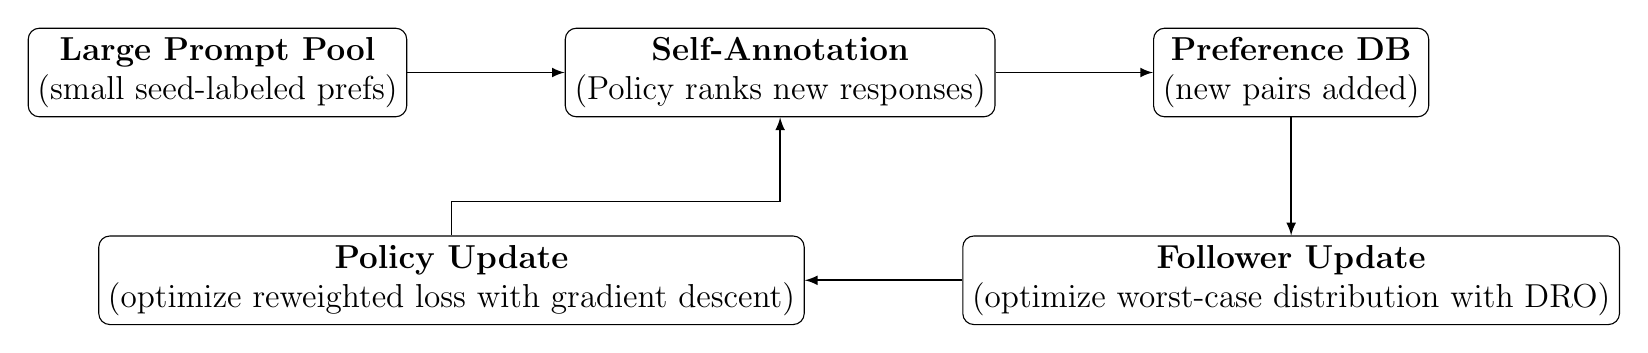
\begin{tikzpicture}[
    font=\large, % <-- Makes text in the nodes larger
    node distance=2.0cm,
    >=latex,
    box/.style={
      rectangle,
      draw=black,
      rounded corners,
      align=center,
      minimum width=2.4cm,
      minimum height=1.1cm
    }
]
\usetikzlibrary{arrows.meta, positioning, calc}

%--- Nodes ---
\node[box] (prompts) {
  \textbf{Large Prompt Pool} \\
  (small seed-labeled prefs)
};
\node[box, right=2.0cm of prompts] (selfanno) {
  \textbf{Self-Annotation} \\
  (Policy ranks new responses)
};
\node[box, right=2.0cm of selfanno] (prefdb) {
  \textbf{Preference DB} \\
  (new pairs added)
};
\node[box, below=1.5cm of prefdb] (dro) {
  \textbf{Follower Update} \\
  (optimize worst-case distribution with DRO)
};
\node[box, left=2.0cm of dro] (policy) {
  \textbf{Policy Update} \\
  (optimize reweighted loss with gradient descent)
};

%--- Arrows ---
\draw[->, line width=0.6pt] (prompts) -- (selfanno);
\draw[->, line width=0.6pt] (selfanno) -- (prefdb);
\draw[->, line width=0.6pt] (prefdb) -- (dro);
\draw[->, line width=0.6pt] (dro) -- (policy);
\draw[->, line width=0.6pt] (policy) -- ++(0,1.0) -| (selfanno);

\end{tikzpicture}%
}
\caption{%
\textbf{SSAPO workflow.} 
We maintain a large prompt pool and a small set of seed-labeled preferences. 
The policy self-annotates new prompts by generating and ranking responses, 
thus expanding the preference database. 
A follower then identifies a worst-case distribution 
for these preferences, 
and the leader (policy) is updated accordingly. 
This process repeats for multiple iterations.
}
\label{fig:ssapo_framework}
\end{figure}

Figure~\ref{fig:ssapo_framework} summarizes the SSAPO workflow. 
Starting with a small seed of human-labeled preferences plus a large unlabeled pool, 
we proceed in the following loop:

\begin{compactenum}
\item \emph{Self-Annotation.}  
  At each iteration, we sample new unlabeled prompts from 
  $\mathcal{D}_{\mathrm{unlabeled}}$ and let the current policy 
  $\pi_{\theta_t}$ generate candidate responses.  The policy \emph{ranks} them 
  to form winner-loser pairs $(y_w,y_l)$, which expand the preference dataset 
  $\mathcal{D}$.  From these, we build $\hat{\xi}_i = R_{\theta_t}(y_w^i) - R_{\theta_t}(y_l^i)$.

\item \emph{Concave Piecewise-Linear Approx.}  
  We fix $K$ and define $\{\ell_k\}_{k=1}^K$ such that 
  $\widetilde{\ell}(\xi) = \max_k \ell_k(\xi)\le -\!\log\,\sigma(\xi)$ 
  (as in Eq.~\eqref{eq:piecewise_concave_ell}).  

\item \emph{Worst-Case Distribution.}  
  We form $\hat{P}_N=\tfrac1N\sum_{i=1}^N \delta_{\hat{\xi}_i}$, 
  then solve Eq.~\eqref{eq:widetilde_dro} with $\widetilde{\ell}$.  
  By Theorem~\ref{thm:worst_case_concave}, the solution is a discrete distribution 
  $P^*_t \in B_\epsilon(\hat{P}_N)$ that \emph{shifts} each $\hat{\xi}_i$ 
  by up to $q_{ik}^{*}/\alpha_{ik}^{*}$, then applies the affine $\ell_k(\cdot)$ 
  and weights $\alpha_{ik}^{*}$.  

\item \emph{Policy Update.}  
  We train $\pi_{\theta}$ on $P^*_t$ by minimizing 
  $\mathbb{E}_{P^*_t}\bigl[-\!\log\,\sigma(R_\theta(y_w)-R_\theta(y_l))\bigr]$.  
  Noting that $P^*_t$ identifies how often each shifted $\xi_i$ is “activated,” 
  we can equivalently reweight the original samples for gradient-based updates.
\end{compactenum}

Repeating for $T$ total iterations yields the final aligned policy $\pi_{\theta_T}$. A more explicit version of SSAPO is provided in Algorithm~\ref{algo:ssapo} (Appendix~\ref{sec:SSAPO_algorithm+analysis}), along with its computational complexity analysis.

\subsubsection{Scalability via Uniform Grouping and Approximation}
\label{subsec:discussion_approx}

\paragraph{Grouping Large Datasets.}
When $N$ is large (e.g.\ $\!10^5\!$ or more preferences), solving the convex program 
in Step~(Worst-Case Distribution) can be expensive.  A popular heuristic partitions 
$\{\hat{\xi}_1,\dots,\hat{\xi}_N\}$ into $M$ groups (each of size $G=N/M$), 
and solves the finite program \eqref{eq:widetilde_dro} separately within each group.   %One may resort to primal-dual or specialized cutting-plane
%methods \citep{Esfahani2018DataDrivenDR}, or use approximate relaxations with 
%entropic regularization \citep{Cuturi2013Sinkhorn}.
The resulting distributions $P^*_m$ are then averaged (or merged proportionally):
$$
P_{\mathrm{final}}^*
\;=\;
\frac{1}{M}
\sum_{m=1}^M
P^*_m.
$$
While not an \emph{exact} solution to the global $N$-sample problem, 
this still confers substantial robustness while reducing complexity from 
$N$ to $G \ll N$ in each subproblem. In summary, this grouping approach greatly reduces memory/compute cost, and is parallelizable.
%Alternatives include \emph{mini-batch} sampling \citep{Blanchet2019quantifying} 
%and \emph{clustering} \citep{Khezeli2019,Gao2022distributionally}.

\begin{remark}[Approximation Effects on SGPO Guarantees]
    Two approximations separate SSAPO from the ideal solution of 
Section~\ref{sec:theory}: (1) \emph{Concave Under-Approximation:}  
 Replacing $-\!\log\,\sigma(\cdot)$ with its piecewise-linear approximation $\widetilde{\ell}(\cdot)$ (i.e., $\widetilde{\ell}(\xi)\le -\!\log\,\sigma(\xi)$) ensures feasibility in Theorem~\ref{thm:worst_case_concave}, but slightly weakens the adversarial effect. Consequently, the policy may be \emph{less robust} than in the fully ideal solution $\max_{P}\!\mathbb{E}_P[-\!\log\,\sigma(\cdot)]$. Increasing $K$ (i.e., refining the linear approximation) narrows this gap. (2)\emph{Partitioned Solver:}   Rather than solving one global $\arg\max_{P \in B_\epsilon(\hat{P}_N)}$, SSAPO partitions the dataset into $M$ groups and separately solves $M$ subproblems. Merging their solutions may deviate from a unified optimum, but it still explores adversarial reweighting in each subgroup, preserving much of SGPO’s robustness against distributional shifts.
\end{remark}

\vspace{-0.1 in}
Despite these approximations, SSAPO preserves the \emph{Stackelberg} essence: the policy is trained against worst-case reweightings within an $\epsilon$-Wasserstein distance. As a result, it retains the key benefit of \emph{bounded regret} for moderate shifts (Theorem~\ref{thm:sgpo_regret}), while remaining computationally tractable. Indeed, if $K \!\to\! \infty$ and $M\!=\!1$, SSAPO recovers the exact follower solution (subject to sampling). Empirically (Section~\ref{sec:experiments}), these approximations still yield substantial label-efficiency and robustness gains over standard DPO.

%\paragraph{Effects on SGPO Guarantees.}
%\begin{enumerate}
%    \item \textbf{Concave Under-Approximation:}  
%      Using $\widetilde{\ell}(\xi)\le -\!\log\,\sigma(\xi)$ ensures feasibility 
%      in Theorem~\ref{thm:worst_case_concave}, but reduces the adversary’s effect.  
%      Hence, the policy may be slightly \emph{less robust} than the ideal solution 
%      of $\max_{P}\mathbb{E}_P[-\!\log\,\sigma(\cdot)]$.  Increasing $K$ 
%      (refining the linear segments) narrows this gap.
%   \item \textbf{Partitioned Solver:}  
%      Instead of one global $\arg\max_{P\in B_\epsilon(\hat{P}_N)}$, 
%      grouping effectively solves $M$ separate subproblems and combines them.  
%      This may deviate from a single unified optimum distribution.  
%      Nonetheless, each partial subproblem still explores adversarial 
%      reweighting, retaining a significant portion of SGPO’s protection 
%      against distributional shifts.
%\end{enumerate}

%Despite these approximations, SSAPO retains the essential \emph{Stackelberg} nature:
%the policy trains against a worst-case reweighting of preferences within 
%\(\epsilon\)-Wasserstein distance.  Consequently, SSAPO still reaps the main %benefits 
%of bounded regret under moderate shifts (Theorem~\ref{thm:sgpo_regret}),
%while ensuring practical feasibility.
%As $K\to\infty$ and $M=1$ (no partitioning), SSAPO recovers the full 
%follower’s solution (subject to the sample-based approximation).  
%In practice, these approximations offer a favorable balance between 
%robustness and computational feasibility.
%Empirical results in Section~\ref{sec:experiments}
%demonstrate label-efficiency and robustness gains relative to standard DPO.

%\section{Experiments}
\label{sec:exp}
Following the settings in Section \ref{sec:existing}, we evaluate \textit{NovelSum}'s correlation with the fine-tuned model performance across 53 IT datasets and compare it with previous diversity metrics. Additionally, we conduct a correlation analysis using Qwen-2.5-7B \cite{yang2024qwen2} as the backbone model, alongside previous LLaMA-3-8B experiments, to further demonstrate the metric's effectiveness across different scenarios. Qwen is used for both instruction tuning and deriving semantic embeddings. Due to resource constraints, we run each strategy on Qwen for two rounds, resulting in 25 datasets. 

\subsection{Main Results}

\begin{table*}[!t]
    \centering
    \resizebox{\linewidth}{!}{
    \begin{tabular}{lcccccccccc}
    \toprule
    \multirow{3}*{\textbf{Diversity Metrics}} & \multicolumn{10}{c}{\textbf{Data Selection Strategies}} \\
    \cmidrule(lr){2-11}
    & \multirow{2}*{\textbf{K-means}} & \multirow{2}*{\vtop{\hbox{\textbf{K-Center}}\vspace{1mm}\hbox{\textbf{-Greedy}}}}  & \multirow{2}*{\textbf{QDIT}} & \multirow{2}*{\vtop{\hbox{\textbf{Repr}}\vspace{1mm}\hbox{\textbf{Filter}}}} & \multicolumn{5}{c}{\textbf{Random}} & \multirow{2}{*}{\textbf{Duplicate}} \\ 
    \cmidrule(lr){6-10}
    & & & & & \textbf{$\mathcal{X}^{all}$} & ShareGPT & WizardLM & Alpaca & Dolly &  \\
    \midrule
    \rowcolor{gray!15} \multicolumn{11}{c}{\textit{LLaMA-3-8B}} \\
    Facility Loc. $_{\times10^5}$ & \cellcolor{BLUE!40} 2.99 & \cellcolor{ORANGE!10} 2.73 & \cellcolor{BLUE!40} 2.99 & \cellcolor{BLUE!20} 2.86 & \cellcolor{BLUE!40} 2.99 & \cellcolor{BLUE!0} 2.83 & \cellcolor{BLUE!30} 2.88 & \cellcolor{BLUE!0} 2.83 & \cellcolor{ORANGE!20} 2.59 & \cellcolor{ORANGE!30} 2.52 \\    
    DistSum$_{cosine}$  & \cellcolor{BLUE!30} 0.648 & \cellcolor{BLUE!60} 0.746 & \cellcolor{BLUE!0} 0.629 & \cellcolor{BLUE!50} 0.703 & \cellcolor{BLUE!10} 0.634 & \cellcolor{BLUE!40} 0.656 & \cellcolor{ORANGE!30} 0.578 & \cellcolor{ORANGE!10} 0.605 & \cellcolor{ORANGE!20} 0.603 & \cellcolor{BLUE!10} 0.634 \\
    Vendi Score $_{\times10^7}$ & \cellcolor{BLUE!30} 1.70 & \cellcolor{BLUE!60} 2.53 & \cellcolor{BLUE!10} 1.59 & \cellcolor{BLUE!50} 2.23 & \cellcolor{BLUE!20} 1.61 & \cellcolor{BLUE!30} 1.70 & \cellcolor{ORANGE!10} 1.44 & \cellcolor{ORANGE!20} 1.32 & \cellcolor{ORANGE!10} 1.44 & \cellcolor{ORANGE!30} 0.05 \\
    \textbf{NovelSum (Ours)} & \cellcolor{BLUE!60} 0.693 & \cellcolor{BLUE!50} 0.687 & \cellcolor{BLUE!30} 0.673 & \cellcolor{BLUE!20} 0.671 & \cellcolor{BLUE!40} 0.675 & \cellcolor{BLUE!10} 0.628 & \cellcolor{BLUE!0} 0.591 & \cellcolor{ORANGE!10} 0.572 & \cellcolor{ORANGE!20} 0.50 & \cellcolor{ORANGE!30} 0.461 \\
    \midrule    
    \textbf{Model Performance} & \cellcolor{BLUE!60}1.32 & \cellcolor{BLUE!50}1.31 & \cellcolor{BLUE!40}1.25 & \cellcolor{BLUE!30}1.05 & \cellcolor{BLUE!20}1.20 & \cellcolor{BLUE!10}0.83 & \cellcolor{BLUE!0}0.72 & \cellcolor{ORANGE!10}0.07 & \cellcolor{ORANGE!20}-0.14 & \cellcolor{ORANGE!30}-1.35 \\
    \midrule
    \midrule
    \rowcolor{gray!15} \multicolumn{11}{c}{\textit{Qwen-2.5-7B}} \\
    Facility Loc. $_{\times10^5}$ & \cellcolor{BLUE!40} 3.54 & \cellcolor{ORANGE!30} 3.42 & \cellcolor{BLUE!40} 3.54 & \cellcolor{ORANGE!20} 3.46 & \cellcolor{BLUE!40} 3.54 & \cellcolor{BLUE!30} 3.51 & \cellcolor{BLUE!10} 3.50 & \cellcolor{BLUE!10} 3.50 & \cellcolor{ORANGE!20} 3.46 & \cellcolor{BLUE!0} 3.48 \\ 
    DistSum$_{cosine}$ & \cellcolor{BLUE!30} 0.260 & \cellcolor{BLUE!60} 0.440 & \cellcolor{BLUE!0} 0.223 & \cellcolor{BLUE!50} 0.421 & \cellcolor{BLUE!10} 0.230 & \cellcolor{BLUE!40} 0.285 & \cellcolor{ORANGE!20} 0.211 & \cellcolor{ORANGE!30} 0.189 & \cellcolor{ORANGE!10} 0.221 & \cellcolor{BLUE!20} 0.243 \\
    Vendi Score $_{\times10^6}$ & \cellcolor{ORANGE!10} 1.60 & \cellcolor{BLUE!40} 3.09 & \cellcolor{BLUE!10} 2.60 & \cellcolor{BLUE!60} 7.15 & \cellcolor{ORANGE!20} 1.41 & \cellcolor{BLUE!50} 3.36 & \cellcolor{BLUE!20} 2.65 & \cellcolor{BLUE!0} 1.89 & \cellcolor{BLUE!30} 3.04 & \cellcolor{ORANGE!30} 0.20 \\
    \textbf{NovelSum (Ours)}  & \cellcolor{BLUE!40} 0.440 & \cellcolor{BLUE!60} 0.505 & \cellcolor{BLUE!20} 0.403 & \cellcolor{BLUE!50} 0.495 & \cellcolor{BLUE!30} 0.408 & \cellcolor{BLUE!10} 0.392 & \cellcolor{BLUE!0} 0.349 & \cellcolor{ORANGE!10} 0.336 & \cellcolor{ORANGE!20} 0.320 & \cellcolor{ORANGE!30} 0.309 \\
    \midrule
    \textbf{Model Performance} & \cellcolor{BLUE!30} 1.06 & \cellcolor{BLUE!60} 1.45 & \cellcolor{BLUE!40} 1.23 & \cellcolor{BLUE!50} 1.35 & \cellcolor{BLUE!20} 0.87 & \cellcolor{BLUE!10} 0.07 & \cellcolor{BLUE!0} -0.08 & \cellcolor{ORANGE!10} -0.38 & \cellcolor{ORANGE!30} -0.49 & \cellcolor{ORANGE!20} -0.43 \\
    \bottomrule
    \end{tabular}
    }
    \caption{Measuring the diversity of datasets selected by different strategies using \textit{NovelSum} and baseline metrics. Fine-tuned model performances (Eq. \ref{eq:perf}), based on MT-bench and AlpacaEval, are also included for cross reference. Darker \colorbox{BLUE!60}{blue} shades indicate higher values for each metric, while darker \colorbox{ORANGE!30}{orange} shades indicate lower values. While data selection strategies vary in performance on LLaMA-3-8B and Qwen-2.5-7B, \textit{NovelSum} consistently shows a stronger correlation with model performance than other metrics. More results are provided in Appendix \ref{app:results}.}
    \label{tbl:main}
    \vspace{-4mm}
\end{table*}


\begin{table}[t!]
\centering
\resizebox{\linewidth}{!}{
\begin{tabular}{lcccc}
\toprule
\multirow{2}*{\textbf{Diversity Metrics}} & \multicolumn{3}{c}{\textbf{LLaMA}} & \textbf{Qwen}\\
\cmidrule(lr){2-4} \cmidrule(lr){5-5} 
& \textbf{Pearson} & \textbf{Spearman} & \textbf{Avg.} & \textbf{Avg.} \\
\midrule
TTR & -0.38 & -0.16 & -0.27 & -0.30 \\
vocd-D & -0.43 & -0.17 & -0.30 & -0.31 \\
\midrule
Facility Loc. & 0.86 & 0.69 & 0.77 & 0.08 \\
Entropy & 0.93 & 0.80 & 0.86 & 0.63 \\
\midrule
LDD & 0.61 & 0.75 & 0.68 & 0.60 \\
KNN Distance & 0.59 & 0.80 & 0.70 & 0.67 \\
DistSum$_{cosine}$ & 0.85 & 0.67 & 0.76 & 0.51 \\
Vendi Score & 0.70 & 0.85 & 0.78 & 0.60 \\
DistSum$_{L2}$ & 0.86 & 0.76 & 0.81 & 0.51 \\
Cluster Inertia & 0.81 & 0.85 & 0.83 & 0.76 \\
Radius & 0.87 & 0.81 & 0.84 & 0.48 \\
\midrule
NovelSum & \textbf{0.98} & \textbf{0.95} & \textbf{0.97} & \textbf{0.90} \\
\bottomrule
\end{tabular}
}
\caption{Correlations between different metrics and model performance on LLaMA-3-8B and Qwen-2.5-7B.  “Avg.” denotes the average correlation (Eq. \ref{eq:cor}).}
\label{tbl:correlations}
\vspace{-2mm}
\end{table}

\paragraph{\textit{NovelSum} consistently achieves state-of-the-art correlation with model performance across various data selection strategies, backbone LLMs, and correlation measures.}
Table \ref{tbl:main} presents diversity measurement results on datasets constructed by mainstream data selection methods (based on $\mathcal{X}^{all}$), random selection from various sources, and duplicated samples (with only $m=100$ unique samples). 
Results from multiple runs are averaged for each strategy.
Although these strategies yield varying performance rankings across base models, \textit{NovelSum} consistently tracks changes in IT performance by accurately measuring dataset diversity. For instance, K-means achieves the best performance on LLaMA with the highest NovelSum score, while K-Center-Greedy excels on Qwen, also correlating with the highest NovelSum. Table \ref{tbl:correlations} shows the correlation coefficients between various metrics and model performance for both LLaMA and Qwen experiments, where \textit{NovelSum} achieves state-of-the-art correlation across different models and measures.

\paragraph{\textit{NovelSum} can provide valuable guidance for data engineering practices.}
As a reliable indicator of data diversity, \textit{NovelSum} can assess diversity at both the dataset and sample levels, directly guiding data selection and construction decisions. For example, Table \ref{tbl:main} shows that the combined data source $\mathcal{X}^{all}$ is a better choice for sampling diverse IT data than other sources. Moreover, \textit{NovelSum} can offer insights through comparative analyses, such as: (1) ShareGPT, which collects data from real internet users, exhibits greater diversity than Dolly, which relies on company employees, suggesting that IT samples from diverse sources enhance dataset diversity \cite{wang2024diversity-logD}; (2) In LLaMA experiments, random selection can outperform some mainstream strategies, aligning with prior work \cite{xia2024rethinking,diddee2024chasing}, highlighting gaps in current data selection methods for optimizing diversity.



\subsection{Ablation Study}


\textit{NovelSum} involves several flexible hyperparameters and variations. In our main experiments, \textit{NovelSum} uses cosine distance to compute $d(x_i, x_j)$ in Eq. \ref{eq:dad}. We set $\alpha = 1$, $\beta = 0.5$, and $K = 10$ nearest neighbors in Eq. \ref{eq:pws} and \ref{eq:dad}. Here, we conduct an ablation study to investigate the impact of these settings based on LLaMA-3-8B.

\begin{table}[ht!]
\centering
\resizebox{\linewidth}{!}{
\begin{tabular}{lccc}
\toprule
\textbf{Variants} & \textbf{Pearson} & \textbf{Spearman} & \textbf{Avg.} \\
\midrule
NovelSum & 0.98 & 0.96 & 0.97 \\
\midrule
\hspace{0.10cm} - Use $L2$ distance & 0.97 & 0.83 & 0.90\textsubscript{↓ 0.08} \\
\hspace{0.10cm} - $K=20$ & 0.98 & 0.96 & 0.97\textsubscript{↓ 0.00} \\
\hspace{0.10cm} - $\alpha=0$ (w/o proximity) & 0.79 & 0.31 & 0.55\textsubscript{↓ 0.42} \\
\hspace{0.10cm} - $\alpha=2$ & 0.73 & 0.88 & 0.81\textsubscript{↓ 0.16} \\
\hspace{0.10cm} - $\beta=0$ (w/o density) & 0.92 & 0.89 & 0.91\textsubscript{↓ 0.07} \\
\hspace{0.10cm} - $\beta=1$ & 0.90 & 0.62 & 0.76\textsubscript{↓ 0.21} \\
\bottomrule
\end{tabular}
}
\caption{Ablation Study for \textit{NovelSum}.}
\label{tbl:ablation}
\vspace{-2mm}
\end{table}

In Table \ref{tbl:ablation}, $\alpha=0$ removes the proximity weights, and $\beta=0$ eliminates the density multiplier. We observe that both $\alpha=0$ and $\beta=0$ significantly weaken the correlation, validating the benefits of the proximity-weighted sum and density-aware distance. Additionally, improper values for $\alpha$ and $\beta$ greatly reduce the metric's reliability, highlighting that \textit{NovelSum} strikes a delicate balance between distances and distribution. Replacing cosine distance with Euclidean distance and using more neighbors for density approximation have minimal impact, particularly on Pearson's correlation, demonstrating \textit{NovelSum}'s robustness to different distance measures.







\section{Experiments}\label{sec:experiments}

\paragraph{Graph subsampling.} We compare our approach with several graph subsampling and condensation methods. KiDD \citep{kidd} and DosCond \citep{jin2022condensing} condense datasets into small synthetic graphs but are not label-agnostic. For a fair comparison, we modify them to operate in a label-agnostic manner by removing their label-aware components in the ``without labels'' section of Tables~\ref{tab:all-results-graph-subsampling1} and \ref{tab:all-results-graph-subsampling2}, as detailed in Appendix~\ref{sec:additional-background-experiments-vallabel}. Since these methods do not support randomized train/test splits and rely on fixed initializations, we do not randomize over splits but do randomize over GNN parameter initializations. MIRAGE \citep{mirage} is another condensation method that subsamples computation trees, but persistent runtime errors in its implementation prevented thorough benchmarking, an issue also reported by \citet{sun2024gc}. We successfully ran MIRAGE on two datasets for certain sampling percentages, as detailed in Appendix~\ref{sec:additional-background-experiments-mirage}.  In addition to these methods, we construct three additional baselines. \emph{WL} applies $k$-medoids clustering using the widely-used Weisfeiler-Lehman (WL) kernel \citep{shervashidze2011weisfeiler}. \emph{Random} performs uniform graph subsampling. \emph{Feature} applies $k$-medoids clustering based only on node features, ignoring graph structure (see Appendix~\ref{sec:additional-background-experiments-feature}). This baseline is particularly useful for evaluating the impact of structure-aware methods such as TMD.  We use an 80/20 train/test split and select between 1\% and 10\% of the training graphs. A GNN is trained on the selected graphs, and we report the average test performance with 95\% confidence intervals over 20 trials with random train/test splits and network initializations.  

Our findings are summarized in Tables~\ref{tab:all-results-graph-subsampling1} and \ref{tab:all-results-graph-subsampling2}. Following \citet{jin2022condensing}, we measure test AUC-ROC on OGBG datasets and classification test accuracy on the remaining datasets. ``Wins'' count how often a method outperforms others, while ``Fails'' count how often a method falls below 50\% accuracy, as all tasks involve binary classification.  TMD consistently ranks first or second across nearly all datasets and subsampling percentages, except on NCI1, where no method outperforms Random. While Random achieves strong performance on NCI1, it performs poorly on most other datasets, a trend also observed with DosCond, which achieves strong results on OGBG-MOLBACE but struggles without labels. Overall, TMD attains the highest total wins across datasets, as shown in Table~\ref{tab:wins-fails-graph}. Additionally, while DosCond and KiDD exhibit high variance, particularly on PROTEINS, TMD maintains stable performance across different subsampling percentages. This consistency is reflected in its low fail count in Table~\ref{tab:wins-fails-graph}, underscoring the robustness of our approach.  

\begin{table}[t]
\caption{Summary of graph and node subsampling performance. The ``Wins" column counts the number of times each method achieves the best test performance across datasets and sampling percentages. The ``Fails" column counts instances where test performance falls below 50\% (worse than random chance). No fails were observed for node subsampling. TMD achieves the highest number of wins across both tasks, while the strong performance of Random is primarily observed on the NCI1 dataset. Full results are presented in Tables~\ref{tab:all-results-graph-subsampling1}, \ref{tab:all-results-graph-subsampling2}, and \ref{tab:combined-results-nodes}.}
\centering
\label{tab:summary}
\begin{tabular}{cc} 
\begin{subtable}{0.48\textwidth}
    \centering
    \caption{Graph subsampling}
    \label{tab:wins-fails-graph}
    \begin{tabular}{l | c | c}
    \hline
    \textbf{Method} & \textbf{Wins} $\uparrow$ & \textbf{Fails} $\downarrow$ \\
    \hline
    DosCond & 11 & 20 \\
    KiDD & 7  & 7 \\
    Feature & 13  & 3 \\
    WL & 8 & 4 \\
    Random & 18 & 7 \\
    \textbf{TMD} & \textbf{23} & \textbf{2} \\
    \hline
    \end{tabular}
\end{subtable}
\begin{subtable}{0.48\textwidth}
    \centering
    \caption{Node subsampling}
    \label{tab:wins-fails-node}
    \begin{tabular}{l | c }
    \hline
    \textbf{Method} & \textbf{Wins} $\uparrow$  \\
    \hline
    RW & 15 \\
    k-cores & 5  \\
    Random & 16 \\
    \textbf{TMD} & \textbf{25} \\
    \hline
    \end{tabular}
\end{subtable}
\end{tabular}
\end{table}


\paragraph{Node subsampling.} To our knowledge, no existing methods focus on node subsampling for graph classification, so we adapt two related approaches as benchmarks. \emph{K-cores}, proposed by \citet{razin2023ability}, is a node selection heuristic based on $k$-core decomposition, which identifies structurally important nodes by iteratively pruning low-degree nodes. \emph{RW}, introduced by \citet{salha2022degeneracy}, is a random-walk-based heuristic originally designed for subgraph sampling in large graph autoencoders. Additionally, we compare against \emph{Random}, which performs uniform node subsampling.  For our proposed node subsampling method (Theorems~\ref{thm:node-subsampling-relaxed} and~\ref{thm:node-subsampling-relaxed-algorithm}), we construct the candidate set $\mathcal{S}$ using breadth-first search (BFS) trees, leveraging the fact that BFS preserves critical motifs in real-world networks~\citep{alimohammadi2023local}. We further augment $\mathcal{S}$ with subsets generated by the RW and k-cores heuristics. The final subset is then selected using TMD. Additional details are provided in Appendix~\ref{sec:heuristic}.  Datasets with relatively larger graphs, such as COX2, PROTEINS, and DD, are well-suited for node subsampling, whereas MUTAG, NCI1, OGBG-MOLBACE, and OGBG-MOLBBBP contain fewer than 35 nodes per graph. For completeness, we include results on MUTAG to demonstrate that our method remains competitive even on smaller graphs.  

Table~\ref{tab:combined-results-nodes} compares test accuracy across these methods for sampling fractions ranging from 10\% to 90\%. We report averages with 95\% confidence intervals over 20 trials with random neural network initializations and train/test splits. The ``W'' row counts the number of times a method outperforms others. TMD consistently ranks among the top two methods and achieves the best overall performance (Table~\ref{tab:wins-fails-node}).  \\

%\newpage
\begin{table}[H]
\centering
\caption{Graph subsampling performance across sampling percentages for TUDatasets, reported as mean ± confidence bar of accuracy (ACC) or area under the ROC (ROC-AUC). Best and second-best per column are in dark/light green, respectively. W is total wins per method.}
\vspace{.1in}
\label{tab:all-results-graph-subsampling1} 
\begin{subtable}{\textwidth}
\captionsetup[subtable]{aboveskip=0pt, belowskip=0pt}
\centering
\resizebox{1.0\textwidth}{!} & \textbf{2\%} & \textbf{3\%} & \textbf{4\%} & \textbf{5\%} & \textbf{6\%} & \textbf{7\%} & \textbf{8\%} & \textbf{9\%} & \textbf{10\%} & \textbf{W} & \textbf{F} \\
\hline
\multicolumn{12}{c}{\textbf{With labels}} \\
\hline
\textbf{Doscond} & 0.66±0.01 & 0.64±0.03 & 0.63±0.00 & 0.68±0.03 & 0.66±0.00 & 0.64±0.01 & 0.65±0.00 & 0.66±0.01 & 0.65±0.00 & 0.66±0.00 & - & 0 \\
\textbf{Kidd} & 0.66±0.03 & 0.68±0.03 & 0.71±0.03 & 0.69±0.03 & 0.70±0.03 & 0.68±0.03 & 0.66±0.02 & 0.64±0.02 & 0.69±0.03 & 0.68±0.03 &  - & 0\\
\hline
\multicolumn{12}{c}{\textbf{Without labels}} \\
\hline
\textbf{Doscond} & 0.48±0.03 & \cellcolor{green!80}{0.67±0.01} & 0.65±0.01 & 0.66±0.00 & 0.55±0.02 & 0.63±0.00 & 0.61±0.01 & 0.65±0.01 & 0.61±0.01 & 0.63±0.01 & 1 & 0\\
\textbf{Kidd} & \cellcolor{green!25}{0.60±0.02} & 0.58±0.02 & 0.55±0.01 & 0.56±0.02 & 0.60±0.02 & 0.61±0.03 & 0.60±0.02 & 0.62±0.02 & 0.58±0.01 & 0.56±0.02 & 0 & 0\\
\textbf{Feature} & 0.57±0.04 & 0.60±0.05 & 0.62±0.03 & 0.65±0.03 & \cellcolor{green!80}{0.67±0.02} & 0.67±0.04 & \cellcolor{green!80}{0.70±0.02} & \cellcolor{green!25}{0.67±0.04} & \cellcolor{green!25}{0.68±0.03} & \cellcolor{green!80}{0.73±0.01} & 3 & 0 \\
\textbf{WL} & \cellcolor{green!25}{0.60±0.03} & 0.62±0.04 & \cellcolor{green!25}{0.67±0.03} & \cellcolor{green!25}{0.68±0.02} & \cellcolor{green!25}{0.65±0.03} & \cellcolor{green!25}{0.68±0.02} & \cellcolor{green!25}{0.69±0.02} & \cellcolor{green!80}{0.69±0.04} & \cellcolor{green!80}{0.69±0.02} & 0.68±0.02 & 2 & 0\\
\textbf{Random} & \cellcolor{green!80}{0.62±0.02} & 0.62±0.02 & 0.63±0.03 & 0.65±0.02 & \cellcolor{green!80}{0.67±0.02} & 0.63±0.03 & 0.67±0.02 & \cellcolor{green!25}{0.67±0.02} & \cellcolor{green!80}{0.69±0.02} & 0.68±0.02 & 3 & 0\\
\textbf{TMD} & \cellcolor{green!80}{0.62±0.02} & \cellcolor{green!25}{0.63±0.03} & \cellcolor{green!80}{0.69±0.02} & \cellcolor{green!80}{0.69±0.02} & \cellcolor{green!80}{0.67±0.02} & \cellcolor{green!80}{0.70±0.02} & 0.67±0.01 & \cellcolor{green!80}{0.69±0.02} & \cellcolor{green!80}{0.69±0.03} & \cellcolor{green!25}{0.71±0.20} & 7 & 0\\
\hline
\end{tabular}
}
\subcaption{COX2. \vspace{-.4cm}}\label{tab:COX2}
\end{subtable}

\vspace{1em}


\begin{subtable}{\textwidth}
\centering
\resizebox{1.0\textwidth}{!}{%
\begin{tabular}{l | c | c | c | c | c | c | c | c | c | c | c | c}

\hline
\multicolumn{12}{c}{\textbf{With labels}} \\
\hline
\textbf{Doscond} & 0.74±0.05 & 0.77±0.02 & 0.78±0.00 & 0.79±0.01 & 0.78±0.01 & 0.78±0.00 & 0.78±0.02 & 0.76±0.03 & 0.78±0.01 & 0.78±0.01 & - & 0 \\
\textbf{Kidd} & 0.17±0.00 & 0.17±0.00 & 0.39±0.31 & 0.83±0.00 & 0.83±0.00 & 0.83±0.00 & 0.83±0.00 & 0.83±0.00 & 0.83±0.00 & 0.39±0.31 &  - & 0 \\
\hline
\multicolumn{12}{c}{\textbf{Without labels}} \\
\hline
\textbf{Doscond} & 0.44±0.14 & 0.22±0.00 & 0.25±0.03 & 0.25±0.03 & 0.77±0.02 & 0.39±0.08 & 0.65±0.09 & 0.22±0.00 & 0.22±0.00 & 0.21±0.00 & 0 & 8\\
\textbf{Kidd} & 0.17±0.00 & \cellcolor{green!80}{0.83±0.00} & 0.17±0.00 & 0.61±0.31 & \cellcolor{green!80}{0.83±0.00} & \cellcolor{green!80}{0.83±0.00} & 0.17±0.00 & 0.17±0.00 & 0.17±0.00 & 0.61±0.31 & 3 & 5\\
\textbf{Feature} & \cellcolor{green!25}{0.65±0.06} & 0.72±0.05 & \cellcolor{green!25}{0.71±0.04} & 0.72±0.02 & \cellcolor{green!25}{0.78±0.01} & 0.75±0.03 & \cellcolor{green!25}{0.74±0.04} & 0.73±0.03 & \cellcolor{green!80}{0.78±0.02} & 0.76±0.02 & 1 & 0 \\
\textbf{WL} & 0.57±0.06 & 0.70±0.04 & \cellcolor{green!80}{0.75±0.02} & \cellcolor{green!25}{0.76±0.02} & 0.77±0.02 & \cellcolor{green!25}{0.77±0.02} & \cellcolor{green!80}{0.77±0.02} & \cellcolor{green!25}{0.77±0.02} & \cellcolor{green!80}{0.78±0.02} & \cellcolor{green!80}{0.78±0.01} & 4 & 0\\
\textbf{Random} & \cellcolor{green!25}{0.65±0.07} & 0.70±0.04 & 0.69±0.05 & 0.68±0.06 & 0.76±0.04 & 0.74±0.04 & \cellcolor{green!25}{0.74±0.03} & 0.74±0.04 & 0.75±0.06 & \cellcolor{green!25}{0.77±0.03} & 0 & 0 \\
\textbf{TMD} & \cellcolor{green!80}{0.70±0.04} & \cellcolor{green!25}{0.76±0.02} & \cellcolor{green!80}{0.75±0.03} & \cellcolor{green!80}{0.78±0.02} & \cellcolor{green!25}{0.78±0.02} & \cellcolor{green!25}{0.77±0.01} & \cellcolor{green!80}{0.77±0.01} & \cellcolor{green!80}{0.78±0.02} & \cellcolor{green!25}{0.77±0.02} & \cellcolor{green!80}{0.78±0.02} & 6 & 0 \\
\hline
\end{tabular}
}
\subcaption{PROTEINS. \vspace{-.4cm}}\label{tab:proteins}
\end{subtable}

\vspace{1em}


\begin{subtable}{\textwidth}
\centering
\resizebox{1.0\textwidth}{!}{%
\begin{tabular}{l | c | c | c | c | c | c | c | c | c | c | c| c} 
\hline
\multicolumn{12}{c}{\textbf{With labels}} \\
\hline
\textbf{Doscond} & 0.71±0.02 & 0.69±0.01 & 0.69±0.03 & 0.70±0.03 & 0.67±0.02 & 0.69±0.03 & 0.70±0.02 & 0.70±0.02 & 0.70±0.01 & 0.69±0.04 & - & 0 \\
\textbf{Kidd} & 0.68±0.00 & 0.68±0.00 & 0.68±0.00 & 0.68±0.00 & 0.68±0.00 & 0.75±0.10 & 0.68±0.00 & 0.68±0.00 & 0.68±0.00 & 0.74±0.04 & - & 0 \\
\hline
\multicolumn{12}{c}{\textbf{Without labels}} \\
\hline
\textbf{Doscond} & \cellcolor{green!25}{0.67±0.00} & \cellcolor{green!80}{0.74±0.03} & \cellcolor{green!80}{0.73±0.01} & \cellcolor{green!80}{0.73±0.01} & \cellcolor{green!25}{0.71±0.01} & \cellcolor{green!25}{0.70±0.01} & 0.70±0.00 & 0.68±0.01 & 0.72±0.01 & 0.70±0.01 & 3 & 0\\
\textbf{Kidd} & \cellcolor{green!80}{0.68±0.00} & 0.68±0.00 & 0.68±0.00 & 0.44±0.17 & 0.68±0.00 & 0.68±0.00 & 0.32±0.00 & 0.70±0.03 & 0.32±0.00 & 0.32±0.00 & 1 & 0\\
\textbf{Feature} & 0.62±0.05 & 0.65±0.06 & 0.67±0.07 & 0.69±0.03 & 0.70±0.04 & 0.68±0.04 & \cellcolor{green!25}{0.72±0.04} & \cellcolor{green!25}{0.71±0.04} & \cellcolor{green!80}{0.74±0.04} & \cellcolor{green!80}{0.74±0.04} & 2 & 3 \\
\textbf{WL} & \cellcolor{green!25}{0.67±0.04} & 0.70±0.04 & \cellcolor{green!25}{0.71±0.02} & \cellcolor{green!25}{0.70±0.03} & \cellcolor{green!25}{0.71±0.03} & \cellcolor{green!25}{0.70±0.03} & 0.68±0.03 & 0.70±0.04 & 0.70±0.04 & \cellcolor{green!80}{0.74±0.04} & 1 & 0\\
\textbf{Random} & 0.62±0.05 & 0.65±0.06 & 0.67±0.07 & 0.69±0.03 & 0.70±0.04 & 0.68±0.04 & \cellcolor{green!25}{0.72±0.04} & \cellcolor{green!25}{0.71±0.04} & \cellcolor{green!80}{0.74±0.04} & \cellcolor{green!80}{0.74±0.04} & 2 & 0\\
\textbf{TMD} & 0.64±0.07 & \cellcolor{green!25}{0.71±0.04} & 0.70±0.03 & \cellcolor{green!80}{0.73±0.04} & \cellcolor{green!80}{0.76±0.04} & \cellcolor{green!80}{0.72±0.05} & \cellcolor{green!80}{0.75±0.04} & \cellcolor{green!80}{0.75±0.03} & \cellcolor{green!25}{0.73±0.04} & \cellcolor{green!25}{0.73±0.03} & 5 & 0\\
\hline
\end{tabular}
}
\subcaption{MUTAG. \vspace{-.4cm}}\label{tab:mutag}
\end{subtable}

\vspace{1em}

\begin{subtable}{\textwidth}
\centering
\resizebox{1.0\textwidth}{!}{%
\begin{tabular}{l | c | c | c | c | c | c | c | c | c | c | c | c}
\hline
\multicolumn{12}{c}{\textbf{With labels}} \\
\hline
\textbf{Doscond} & 0.56±0.01 & 0.56±0.02 & 0.57±0.02 & 0.58±0.02 & 0.58±0.02 & 0.56±0.03 & 0.59±0.02 & 0.61±0.02 & 0.61±0.02 & 0.61±0.02 & - & 0\\
\textbf{Kidd} & 0.60±0.01 & 0.60±0.01 & 0.61±0.02 & 0.61±0.01 & 0.61±0.02 & 0.62±0.02 & 0.62±0.01 & 0.62±0.01 & 0.62±0.01 & 0.62±0.01 & - & 0 \\
\hline
\multicolumn{12}{c}{\textbf{Without labels}} \\
\hline
\textbf{Doscond} & 0.50±0.02 & 0.51±0.03 & 0.49±0.03 & 0.52±0.03 & 0.52±0.02 & 0.54±0.02 & 0.54±0.02 & 0.54±0.02 & 0.51±0.04 & 0.55±0.03 & 0 & 0\\
\textbf{Kidd} & \cellcolor{green!80}{0.55±0.03} & \cellcolor{green!25}{0.56±0.03} & \cellcolor{green!25}{0.56±0.03} & \cellcolor{green!25}{0.54±0.05} & \cellcolor{green!25}{0.57±0.02} & \cellcolor{green!25}{0.57±0.02} & \cellcolor{green!25}{0.57±0.02} & \cellcolor{green!25}{0.57±0.02} & \cellcolor{green!25}{0.58±0.02} & \cellcolor{green!25}{0.58±0.02} & 1 & 0\\
\textbf{Feature} & \cellcolor{green!25}{0.51±0.01} & 0.53±0.01 & 0.52±0.01 & 0.53±0.02 & 0.53±0.02 & 0.53±0.02 & 0.54±0.02 & 0.53±0.01 & 0.56±0.03 & 0.54±0.03 & 0 & 0\\
\textbf{WL} & \cellcolor{green!25}{0.51±0.01} & 0.51±0.01 & 0.52±0.01 & 0.50±0.01 & 0.51±0.01 & 0.51±0.01 & 0.50±0.00 & 0.51±0.01 & 0.52±0.01 & 0.53±0.02 & 0 & 0\\
\textbf{Random} & \cellcolor{green!80}{0.55±0.02} & \cellcolor{green!80}{0.59±0.02} & \cellcolor{green!80}{0.62±0.01} & \cellcolor{green!80}{0.60±0.02} & \cellcolor{green!80}{0.63±0.02} & \cellcolor{green!80}{0.62±0.02} & \cellcolor{green!80}{0.61±0.02} & \cellcolor{green!80}{0.61±0.02} & \cellcolor{green!80}{0.64±0.01} & \cellcolor{green!80}{0.65±0.01} & 10 & 0\\
\textbf{TMD} & \cellcolor{green!25}{0.51±0.01} & 0.53±0.01 & 0.52±0.01 & 0.53±0.02 & 0.53±0.02 & 0.53±0.02 & 0.54±0.02 & 0.53±0.01 & 0.56±0.03 & 0.54±0.03 & 0 & 0\\
\hline
\end{tabular}
}
\subcaption{NCI1.\vspace{-.4cm}}\label{tab:NCI1}
\end{subtable}

\end{table}































\clearpage
\newpage

\begin{table}[t!]
\centering
\caption{Graph subsampling performance across sampling percentages for OGBG datasets, reported as mean ± confidence bar of accuracy (ACC) or area under the ROC (ROC-AUC). Best and second-best per column are in dark/light green, respectively. W is total wins per method.}
\vspace{.1in}
\label{tab:all-results-graph-subsampling2} 




\begin{subtable}{\textwidth}
\centering
\resizebox{1.0\textwidth}{!}{%
\begin{tabular}{l | c | c | c | c | c | c | c | c | c | c | c | c}

\hline
\multicolumn{12}{c}{\textbf{With labels}} \\
\hline
\textbf{Doscond} & 0.51±0.01 & 0.51±0.02 & 0.52±0.02 & 0.52±0.02 & 0.40±0.02 & 0.54±0.02 & 0.55±0.02 & 0.56±0.02 & 0.58±0.02 & 0.62±0.02 & - & 0 \\
\textbf{Kidd} & 0.62±0.02 & 0.62±0.04 & 0.62±0.05 & 0.62±0.06 & 0.62±0.07 & 0.58±0.15 & 0.62±0.08 & 0.63±0.10 & 0.63±0.11 & 0.63±0.12 & - & 0 \\
\hline
\multicolumn{12}{c}{\textbf{Without labels}} \\
\hline
\textbf{Doscond} & 0.43±0.02 & 0.44±0.02 & 0.30±0.02 & 0.45±0.02 & 0.46±0.03 & 0.46±0.03 & 0.32±0.01 & 0.47±0.03 & 0.47±0.04 & 0.48±0.03 & 0 & 10\\
\textbf{Kidd} & 0.57±0.04 & 0.57±0.05 & 0.58±0.04 & 0.58±0.05 & 0.58±0.06 & 0.58±0.05 & 0.58±0.06 & 0.59±0.07 & 0.59±0.07 & 0.59±0.08 & 0 & 0\\
\textbf{Feature} & \cellcolor{green!80}{0.78±0.01} & \cellcolor{green!80}{0.76±0.01} & \cellcolor{green!25}{0.76±0.04} & \cellcolor{green!80}{0.77±0.00} & \cellcolor{green!80}{0.79±0.00} & 0.77±0.01 & \cellcolor{green!25}{0.76±0.01} & \cellcolor{green!25}{0.76±0.00} & \cellcolor{green!80}{0.78±0.00} & \cellcolor{green!80}{0.78±0.01} & 6 & 0\\
\textbf{WL} & 0.57±0.08 & 0.69±0.05 & 0.73±0.06 & 0.74±0.05 & 0.76±0.01 & 0.77±0.01 & 0.72±0.06 & 0.70±0.07 & \cellcolor{green!80}{0.78±0.01} & 0.76±0.01 & 1 & 0\\
\textbf{Random} & 0.62±0.09 & \cellcolor{green!80}{0.76±0.02} & \cellcolor{green!80}{0.77±0.01} & \cellcolor{green!25}{0.76±0.01} & \cellcolor{green!25}{0.77±0.00} & \cellcolor{green!25}{0.78±0.00} & \cellcolor{green!25}{0.76±0.03} & \cellcolor{green!80}{0.77±0.00} & \cellcolor{green!25}{0.77±0.00} & \cellcolor{green!25}{0.77±0.00} & 3 & 0\\
\textbf{TMD} & \cellcolor{green!25}{0.69±0.05} & \cellcolor{green!25}{0.75±0.03} & \cellcolor{green!25}{0.76±0.02} & \cellcolor{green!25}{0.76±0.01} & 0.73±0.04 & \cellcolor{green!80}{0.79±0.02} & \cellcolor{green!80}{0.78±0.01} & \cellcolor{green!80}{0.77±0.01} & \cellcolor{green!25}{0.77±0.01} & 0.73±0.07 & 3 & 0\\
\hline
\end{tabular}
}
\subcaption{OGBG-MOLBBBP. \vspace{-.4cm}}\label{tab:molbbbp}
\end{subtable}
\vspace{1em}

\begin{subtable}{\textwidth}
\centering
\resizebox{1.0\textwidth}{!}{
\begin{tabular}{l | c | c | c | c | c | c | c | c | c | c | c | c}
\hline
\textbf{Doscond} & 0.67±0.01 & 0.67±0.03 & 0.64±0.01 & 0.67±0.01 & 0.65±0.03 & 0.68±0.02 & 0.66±0.02 & 0.67±0.01 & 0.67±0.04 & 0.66±0.02 & - & 0 \\
\textbf{Kidd} & 0.64±0.03 & 0.66±0.03 & 0.65±0.03 & 0.64±0.03 & 0.61±0.03 & 0.63±0.03 & 0.66±0.03 & 0.67±0.03 & 0.69±0.03 & 0.68±0.03 & - & 0 \\
\hline
\multicolumn{12}{c}{\textbf{Without labels}} \\
\hline
\textbf{Doscond} & \cellcolor{green!80}{0.53±0.02} & 0.45±0.04 & \cellcolor{green!80}{0.64±0.03} & \cellcolor{green!80}{0.60±0.02} & 0.37±0.01 & \cellcolor{green!80}{0.56±0.06} & \cellcolor{green!80}{0.61±0.02} & 0.54±0.01 & \cellcolor{green!80}{0.59±0.03} & \cellcolor{green!80}{0.62±0.03} & 7 & 2\\
\textbf{Kidd} & \cellcolor{green!80}{0.53±0.03} & \cellcolor{green!25}{0.51±0.03} & 0.46±0.02 & 0.48±0.02 & \cellcolor{green!80}{0.56±0.03} & \cellcolor{green!25}{0.54±0.03} & \cellcolor{green!25}{0.58±0.03} & 0.55±0.02 & 0.50±0.03 & 0.52±0.03 & 2 & 2\\
\textbf{Feature} & \cellcolor{green!25}{0.50±0.03} & \cellcolor{green!80}{0.52±0.03} & 0.53±0.02 & \cellcolor{green!25}{0.55±0.02} & \cellcolor{green!25}{0.55±0.02} & 0.51±0.02 & 0.55±0.02 & \cellcolor{green!25}{0.56±0.03} & 0.56±0.02 & 0.56±0.02 & 1 & 0\\
\textbf{WL} & 0.48±0.01 & 0.49±0.02 & 0.48±0.02 & 0.51±0.03 & 0.48±0.02 & 0.50±0.02 & 0.53±0.03 & 0.50±0.03 & 0.55±0.03 & 0.53±0.03 & 0 & 4 \\
\textbf{Random} & 0.49±0.02 & 0.49±0.03 & 0.51±0.03 & 0.49±0.02 & 0.48±0.03 & 0.50±0.04 & 0.48±0.02 & 0.48±0.02 & 0.49±0.03 & 0.51±0.03 & 0 & 7\\
\textbf{TMD} & 0.45±0.01 & \cellcolor{green!80}{0.52±0.03} & \cellcolor{green!25}{0.55±0.04} & 0.49±0.02 & 0.54±0.03 & \cellcolor{green!25}{0.54±0.03} & \cellcolor{green!25}{0.58±0.03} & \cellcolor{green!80}{0.60±0.03} & \cellcolor{green!25}{0.57±0.02} & \cellcolor{green!25}{0.58±0.02} & 2 & 2\\
\hline
\end{tabular}
}
\subcaption{OGBG-MOLBACE. \vspace{-.4cm}}\label{tab:molbace}
\end{subtable}
\vspace{1em}


\end{table}



















\begin{table}[H]
\scriptsize
\caption{Node subsampling performance across datasets and sampling percentages, reported as mean ± confidence bar of accuracy (ACC). Best and second-best per column are in dark and light green, respectively. W is total wins per method.}
\label{tab:combined-results-nodes}
\vspace{0.1in}
\centering

\begin{subtable}{\textwidth}
\centering
\resizebox{1.0\textwidth}{!} & \textbf{2\%} & \textbf{3\%} & \textbf{4\%} & \textbf{5\%} & \textbf{6\%} & \textbf{7\%} & \textbf{8\%} & \textbf{9\%} & \textbf{W} \\
\hline
\textbf{RW}
    & \cellcolor{green!80}{0.68±0.02}
    & \cellcolor{green!80}{0.67±0.03}
    & 0.66±0.03
    & 0.65±0.04
    & 0.66±0.04
    & 0.68±0.08
    & 0.71±0.05
    & \cellcolor{green!25}{0.77±0.03}
    & 0.80±0.04
    & 2 \\
\textbf{k-cores}
    & 0.56±0.07
    & \cellcolor{green!25}{0.63±0.04}
    & 0.48±0.07
    & 0.64±0.06
    & \cellcolor{green!25}{0.67±0.05}
    & 0.65±0.06
    & \cellcolor{green!25}{0.73±0.04}
    & 0.73±0.03
    & 0.74±0.03
    & 0 \\
\textbf{Random}
    & \cellcolor{green!80}{0.68±0.04}
    & \cellcolor{green!80}{0.67±0.03}
    & \cellcolor{green!80}{0.70±0.03}
    & \cellcolor{green!80}{0.71±0.03}
    & 0.66±0.03
    & \cellcolor{green!25}{0.69±0.03}
    & \cellcolor{green!80}{0.74±0.03}
    & 0.75±0.03
    & \cellcolor{green!25}{0.81±0.04}
    & 4 \\
\textbf{TMD}
    & \cellcolor{green!25}{0.66±0.05}
    & \cellcolor{green!80}{0.67±0.03}
    & \cellcolor{green!25}{0.68±0.04}
    & \cellcolor{green!25}{0.69±0.02}
    & \cellcolor{green!80}{0.68±0.04}
    & \cellcolor{green!80}{0.72±0.03}
    & \cellcolor{green!80}{0.74±0.04}
    & \cellcolor{green!80}{0.78±0.03}
    & \cellcolor{green!80}{0.84±0.02}
    & 6 \\
\hline
\end{tabular}
}
\caption{MUTAG}
\label{tab:mutag-pivot}
\end{subtable}

\vspace{0em}


\begin{subtable}{\textwidth}
\centering
\resizebox{1.0\textwidth}{!}{%
\begin{tabular}{l|c|c|c|c|c|c|c|c|c|c}

\hline
\textbf{RW}
    & \cellcolor{green!80}{0.61±0.01}
    & \cellcolor{green!80}{0.60±0.01}
    & \cellcolor{green!80}{0.63±0.01}
    & 0.63±0.01
    & \cellcolor{green!25}{0.67±0.02}
    & \cellcolor{green!25}{0.69±0.01}
    & \cellcolor{green!25}{0.68±0.02}
    & \cellcolor{green!80}{0.72±0.01}
    & 0.70±0.02
    & 4 \\
\textbf{k-cores}
    & 0.59±0.01
    & \cellcolor{green!80}{0.60±0.01}
    & 0.60±0.01
    & \cellcolor{green!25}{0.64±0.02}
    & 0.65±0.01
    & \cellcolor{green!25}{0.69±0.02}
    & \cellcolor{green!25}{0.68±0.02}
    & 0.70±0.01
    & \cellcolor{green!25}{0.71±0.01}
    & 1 \\
\textbf{Random}
    & \cellcolor{green!25}{0.60±0.01}
    & \cellcolor{green!80}{0.60±0.01}
    & \cellcolor{green!25}{0.62±0.02}
    & \cellcolor{green!25}{0.64±0.02}
    & \cellcolor{green!25}{0.67±0.02}
    & 0.68±0.01
    & \cellcolor{green!80}{0.71±0.01}
    & 0.70±0.02
    & 0.70±0.02
    & 2 \\
\textbf{TMD}
    & \cellcolor{green!25}{0.60±0.01}
    & \cellcolor{green!80}{0.60±0.01}
    & \cellcolor{green!80}{0.63±0.01}
    & \cellcolor{green!80}{0.65±0.01}
    & \cellcolor{green!80}{0.68±0.01}
    & \cellcolor{green!80}{0.70±0.01}
    & \cellcolor{green!80}{0.71±0.01}
    & \cellcolor{green!25}{0.71±0.01}
    & \cellcolor{green!80}{0.73±0.01}
    & 7 \\
\hline
\end{tabular}
}
\caption{PROTEINS}
\label{tab:proteins-pivot}
\end{subtable}

\vspace{0em}

\begin{subtable}{\textwidth}
\centering
\resizebox{1.0\textwidth}{!}{%
\begin{tabular}{l|c|c|c|c|c|c|c|c|c|c}

\hline
\textbf{RW}
    & \cellcolor{green!25}{0.58±0.01}
    & \cellcolor{green!80}{0.59±0.01}
    & \cellcolor{green!80}{0.61±0.01}
    & 0.63±0.01
    & \cellcolor{green!80}{0.66±0.02}
    & \cellcolor{green!80}{0.69±0.01}
    & \cellcolor{green!80}{0.72±0.02}
    & \cellcolor{green!25}{0.73±0.02}
    & \cellcolor{green!25}{0.74±0.02}
    & 5 \\
\textbf{k-cores}
    & \cellcolor{green!80}{0.59±0.01}
    & \cellcolor{green!80}{0.59±0.01}
    & \cellcolor{green!25}{0.59±0.02}
    & 0.59±0.01
    & 0.60±0.01
    & \cellcolor{green!25}{0.59±0.01}
    & 0.59±0.01
    & 0.60±0.01
    & 0.59±0.01
    & 2 \\
\textbf{Random}
    & \cellcolor{green!80}{0.59±0.01}
    & \cellcolor{green!25}{0.58±0.01}
    & \cellcolor{green!80}{0.61±0.01}
    & \cellcolor{green!25}{0.64±0.01}
    & \cellcolor{green!80}{0.66±0.02}
    & \cellcolor{green!80}{0.69±0.02}
    & \cellcolor{green!25}{0.71±0.02}
    & \cellcolor{green!25}{0.73±0.02}
    & 0.73±0.03
    & 7 \\
\textbf{TMD}
    & \cellcolor{green!25}{0.58±0.02}
    & \cellcolor{green!80}{0.59±0.01}
    & \cellcolor{green!80}{0.61±0.01}
    & \cellcolor{green!80}{0.65±0.02}
    & \cellcolor{green!25}{0.65±0.02}
    & \cellcolor{green!80}{0.69±0.02}
    & 0.70±0.02
    & \cellcolor{green!80}{0.74±0.01}
    & \cellcolor{green!80}{0.76±0.01}
    & 6 \\
\hline
\end{tabular}
}
\caption{DD}
\label{tab:dd-pivot}
\end{subtable}

\vspace{0em}


\begin{subtable}{\textwidth}
\centering
\resizebox{1.0\textwidth}{!}{%
\begin{tabular}{l|c|c|c|c|c|c|c|c|c|c}

\hline
\textbf{RW}
    & \cellcolor{green!25}{0.78±0.01}
    & 0.77±0.01
    & \cellcolor{green!80}{0.79±0.01}
    & \cellcolor{green!80}{0.80±0.02}
    & \cellcolor{green!80}{0.79±0.02}
    & \cellcolor{green!80}{0.78±0.02}
    & \cellcolor{green!25}{0.79±0.02}
    & \cellcolor{green!25}{0.79±0.02}
    & 0.77±0.02
    & 4 \\
\textbf{k-cores}
    & \cellcolor{green!25}{0.78±0.01}
    & \cellcolor{green!25}{0.78±0.02}
    & 0.77±0.01
    & \cellcolor{green!25}{0.79±0.02}
    & 0.74±0.05
    & \cellcolor{green!80}{0.78±0.01}
    & 0.77±0.02
    & 0.78±0.02
    & \cellcolor{green!80}{0.79±0.02}
    & 2 \\
\textbf{Random}
    & \cellcolor{green!80}{0.79±0.02}
    & \cellcolor{green!25}{0.78±0.02}
    & \cellcolor{green!25}{0.78±0.01}
    & \cellcolor{green!25}{0.79±0.02}
    & \cellcolor{green!80}{0.79±0.01}
    & \cellcolor{green!80}{0.78±0.02}
    & 0.77±0.02
    & 0.78±0.01
    & \cellcolor{green!25}{0.78±0.01}
    & 3 \\
\textbf{TMD}
    & \cellcolor{green!80}{0.79±0.02}
    & \cellcolor{green!80}{0.79±0.02}
    & \cellcolor{green!25}{0.78±0.01}
    & 0.77±0.02
    & \cellcolor{green!25}{0.78±0.01}
    & \cellcolor{green!80}{0.78±0.02}
    & \cellcolor{green!80}{0.80±0.02}
    & \cellcolor{green!80}{0.80±0.01}
    & \cellcolor{green!80}{0.79±0.02}
    & 6 \\
\hline
\end{tabular}
}
\caption{COX2}
\label{tab:cox2-pivot}
\end{subtable}

\end{table}


%\FloatBarrier



\section{Conclusion}
In this work, we propose a simple yet effective approach, called SMILE, for graph few-shot learning with fewer tasks. Specifically, we introduce a novel dual-level mixup strategy, including within-task and across-task mixup, for enriching the diversity of nodes within each task and the diversity of tasks. Also, we incorporate the degree-based prior information to learn expressive node embeddings. Theoretically, we prove that SMILE effectively enhances the model's generalization performance. Empirically, we conduct extensive experiments on multiple benchmarks and the results suggest that SMILE significantly outperforms other baselines, including both in-domain and cross-domain few-shot settings.

% \section*{Impact statement}

This paper proposes that machine learning can and should be used to maximize social welfare. In principle, and by construction, the impact of our proposed framework on society aims to be positive. But our paper also points to the inherent difficulties of identifying, and making formal, what `good for society' is. We lean on the field of welfare economics, which has for decades contended with this challenge, for ideas on how the learning community can begin to approach this daunting task.
However, even if these ideas are conceptually appealing,
the path to practical welfare improvement presents many challenges---%
some expected, others unforseen.
% and will likely include many ups and downs.
For example, we may specify incorrect social welfare functions;
or we may specify them correctly but be unable to optimize them appropriately;
or we may be able to optimize but find that 
our assumptions are wrong, that theory differs from practice,
or that there were other considerations and complexities that we did not take into account.
For this we can look to other related fields---%
such as fairness, privacy, and alignment in machine learning---%
which have taken (and are still taking) similar journeys,
and learn from both their success and mistakes.
% and hope that ours will be similar.

Any discipline that seeks to affect policy should do so with much deliberation and care. Whereas welfare economics was designed with the explicit purpose of supporting (and influencing) policymakers,
machine learning has found itself in a similar position, but likely without any planned intent.
On the one hand, adjusting machine learning to support notions, such as social welfare,
that it was not designed to support initially can prove challenging.
However, and as we argue throughout, we believe that building on top of existing machinery is a more practical approach than to begin from scratch.
The necessity of confronting with welfare consideration can also
be an opportunity---as we can leverage these novel challenges
to make machine learning practice more informed, transparent, responsible, and socially aware.


% At the same time, the novelty of the challenges that welfare considerations present to the field make this an opportunity---%
% for chaning the role of machine learning in society for the better in a manner that is informed, transparent, and aware.



\section*{Impact Statement}
Our work aims to improve the data efficiency and robustness of language model alignment by formulating preference optimization as a Stackelberg game and introducing a self-annotation mechanism.  By reducing reliance on large-scale human-labeled data, our framework could democratize alignment research and make it more accessible to smaller organizations, labs, and communities (those lack substantial annotation budgets). Moreover, robust optimization against noisy or adversarial preference distributions may help mitigate unintentional bias if the seed data deviate from the true user preference distribution.




% In the unusual situation where you want a paper to appear in the
% references without citing it in the main text, use \nocite

\bibliography{example_paper}
\bibliographystyle{icml2025}


%%%%%%%%%%%%%%%%%%%%%%%%%%%%%%%%%%%%%%%%%%%%%%%%%%%%%%%%%%%%%%%%%%%%%%%%%%%%%%%
%%%%%%%%%%%%%%%%%%%%%%%%%%%%%%%%%%%%%%%%%%%%%%%%%%%%%%%%%%%%%%%%%%%%%%%%%%%%%%%
% APPENDIX
%%%%%%%%%%%%%%%%%%%%%%%%%%%%%%%%%%%%%%%%%%%%%%%%%%%%%%%%%%%%%%%%%%%%%%%%%%%%%%%
%%%%%%%%%%%%%%%%%%%%%%%%%%%%%%%%%%%%%%%%%%%%%%%%%%%%%%%%%%%%%%%%%%%%%%%%%%%%%%%
\newpage
\appendix
\onecolumn

\subsection{Lloyd-Max Algorithm}
\label{subsec:Lloyd-Max}
For a given quantization bitwidth $B$ and an operand $\bm{X}$, the Lloyd-Max algorithm finds $2^B$ quantization levels $\{\hat{x}_i\}_{i=1}^{2^B}$ such that quantizing $\bm{X}$ by rounding each scalar in $\bm{X}$ to the nearest quantization level minimizes the quantization MSE. 

The algorithm starts with an initial guess of quantization levels and then iteratively computes quantization thresholds $\{\tau_i\}_{i=1}^{2^B-1}$ and updates quantization levels $\{\hat{x}_i\}_{i=1}^{2^B}$. Specifically, at iteration $n$, thresholds are set to the midpoints of the previous iteration's levels:
\begin{align*}
    \tau_i^{(n)}=\frac{\hat{x}_i^{(n-1)}+\hat{x}_{i+1}^{(n-1)}}2 \text{ for } i=1\ldots 2^B-1
\end{align*}
Subsequently, the quantization levels are re-computed as conditional means of the data regions defined by the new thresholds:
\begin{align*}
    \hat{x}_i^{(n)}=\mathbb{E}\left[ \bm{X} \big| \bm{X}\in [\tau_{i-1}^{(n)},\tau_i^{(n)}] \right] \text{ for } i=1\ldots 2^B
\end{align*}
where to satisfy boundary conditions we have $\tau_0=-\infty$ and $\tau_{2^B}=\infty$. The algorithm iterates the above steps until convergence.

Figure \ref{fig:lm_quant} compares the quantization levels of a $7$-bit floating point (E3M3) quantizer (left) to a $7$-bit Lloyd-Max quantizer (right) when quantizing a layer of weights from the GPT3-126M model at a per-tensor granularity. As shown, the Lloyd-Max quantizer achieves substantially lower quantization MSE. Further, Table \ref{tab:FP7_vs_LM7} shows the superior perplexity achieved by Lloyd-Max quantizers for bitwidths of $7$, $6$ and $5$. The difference between the quantizers is clear at 5 bits, where per-tensor FP quantization incurs a drastic and unacceptable increase in perplexity, while Lloyd-Max quantization incurs a much smaller increase. Nevertheless, we note that even the optimal Lloyd-Max quantizer incurs a notable ($\sim 1.5$) increase in perplexity due to the coarse granularity of quantization. 

\begin{figure}[h]
  \centering
  \includegraphics[width=0.7\linewidth]{sections/figures/LM7_FP7.pdf}
  \caption{\small Quantization levels and the corresponding quantization MSE of Floating Point (left) vs Lloyd-Max (right) Quantizers for a layer of weights in the GPT3-126M model.}
  \label{fig:lm_quant}
\end{figure}

\begin{table}[h]\scriptsize
\begin{center}
\caption{\label{tab:FP7_vs_LM7} \small Comparing perplexity (lower is better) achieved by floating point quantizers and Lloyd-Max quantizers on a GPT3-126M model for the Wikitext-103 dataset.}
\begin{tabular}{c|cc|c}
\hline
 \multirow{2}{*}{\textbf{Bitwidth}} & \multicolumn{2}{|c|}{\textbf{Floating-Point Quantizer}} & \textbf{Lloyd-Max Quantizer} \\
 & Best Format & Wikitext-103 Perplexity & Wikitext-103 Perplexity \\
\hline
7 & E3M3 & 18.32 & 18.27 \\
6 & E3M2 & 19.07 & 18.51 \\
5 & E4M0 & 43.89 & 19.71 \\
\hline
\end{tabular}
\end{center}
\end{table}

\subsection{Proof of Local Optimality of LO-BCQ}
\label{subsec:lobcq_opt_proof}
For a given block $\bm{b}_j$, the quantization MSE during LO-BCQ can be empirically evaluated as $\frac{1}{L_b}\lVert \bm{b}_j- \bm{\hat{b}}_j\rVert^2_2$ where $\bm{\hat{b}}_j$ is computed from equation (\ref{eq:clustered_quantization_definition}) as $C_{f(\bm{b}_j)}(\bm{b}_j)$. Further, for a given block cluster $\mathcal{B}_i$, we compute the quantization MSE as $\frac{1}{|\mathcal{B}_{i}|}\sum_{\bm{b} \in \mathcal{B}_{i}} \frac{1}{L_b}\lVert \bm{b}- C_i^{(n)}(\bm{b})\rVert^2_2$. Therefore, at the end of iteration $n$, we evaluate the overall quantization MSE $J^{(n)}$ for a given operand $\bm{X}$ composed of $N_c$ block clusters as:
\begin{align*}
    \label{eq:mse_iter_n}
    J^{(n)} = \frac{1}{N_c} \sum_{i=1}^{N_c} \frac{1}{|\mathcal{B}_{i}^{(n)}|}\sum_{\bm{v} \in \mathcal{B}_{i}^{(n)}} \frac{1}{L_b}\lVert \bm{b}- B_i^{(n)}(\bm{b})\rVert^2_2
\end{align*}

At the end of iteration $n$, the codebooks are updated from $\mathcal{C}^{(n-1)}$ to $\mathcal{C}^{(n)}$. However, the mapping of a given vector $\bm{b}_j$ to quantizers $\mathcal{C}^{(n)}$ remains as  $f^{(n)}(\bm{b}_j)$. At the next iteration, during the vector clustering step, $f^{(n+1)}(\bm{b}_j)$ finds new mapping of $\bm{b}_j$ to updated codebooks $\mathcal{C}^{(n)}$ such that the quantization MSE over the candidate codebooks is minimized. Therefore, we obtain the following result for $\bm{b}_j$:
\begin{align*}
\frac{1}{L_b}\lVert \bm{b}_j - C_{f^{(n+1)}(\bm{b}_j)}^{(n)}(\bm{b}_j)\rVert^2_2 \le \frac{1}{L_b}\lVert \bm{b}_j - C_{f^{(n)}(\bm{b}_j)}^{(n)}(\bm{b}_j)\rVert^2_2
\end{align*}

That is, quantizing $\bm{b}_j$ at the end of the block clustering step of iteration $n+1$ results in lower quantization MSE compared to quantizing at the end of iteration $n$. Since this is true for all $\bm{b} \in \bm{X}$, we assert the following:
\begin{equation}
\begin{split}
\label{eq:mse_ineq_1}
    \tilde{J}^{(n+1)} &= \frac{1}{N_c} \sum_{i=1}^{N_c} \frac{1}{|\mathcal{B}_{i}^{(n+1)}|}\sum_{\bm{b} \in \mathcal{B}_{i}^{(n+1)}} \frac{1}{L_b}\lVert \bm{b} - C_i^{(n)}(b)\rVert^2_2 \le J^{(n)}
\end{split}
\end{equation}
where $\tilde{J}^{(n+1)}$ is the the quantization MSE after the vector clustering step at iteration $n+1$.

Next, during the codebook update step (\ref{eq:quantizers_update}) at iteration $n+1$, the per-cluster codebooks $\mathcal{C}^{(n)}$ are updated to $\mathcal{C}^{(n+1)}$ by invoking the Lloyd-Max algorithm \citep{Lloyd}. We know that for any given value distribution, the Lloyd-Max algorithm minimizes the quantization MSE. Therefore, for a given vector cluster $\mathcal{B}_i$ we obtain the following result:

\begin{equation}
    \frac{1}{|\mathcal{B}_{i}^{(n+1)}|}\sum_{\bm{b} \in \mathcal{B}_{i}^{(n+1)}} \frac{1}{L_b}\lVert \bm{b}- C_i^{(n+1)}(\bm{b})\rVert^2_2 \le \frac{1}{|\mathcal{B}_{i}^{(n+1)}|}\sum_{\bm{b} \in \mathcal{B}_{i}^{(n+1)}} \frac{1}{L_b}\lVert \bm{b}- C_i^{(n)}(\bm{b})\rVert^2_2
\end{equation}

The above equation states that quantizing the given block cluster $\mathcal{B}_i$ after updating the associated codebook from $C_i^{(n)}$ to $C_i^{(n+1)}$ results in lower quantization MSE. Since this is true for all the block clusters, we derive the following result: 
\begin{equation}
\begin{split}
\label{eq:mse_ineq_2}
     J^{(n+1)} &= \frac{1}{N_c} \sum_{i=1}^{N_c} \frac{1}{|\mathcal{B}_{i}^{(n+1)}|}\sum_{\bm{b} \in \mathcal{B}_{i}^{(n+1)}} \frac{1}{L_b}\lVert \bm{b}- C_i^{(n+1)}(\bm{b})\rVert^2_2  \le \tilde{J}^{(n+1)}   
\end{split}
\end{equation}

Following (\ref{eq:mse_ineq_1}) and (\ref{eq:mse_ineq_2}), we find that the quantization MSE is non-increasing for each iteration, that is, $J^{(1)} \ge J^{(2)} \ge J^{(3)} \ge \ldots \ge J^{(M)}$ where $M$ is the maximum number of iterations. 
%Therefore, we can say that if the algorithm converges, then it must be that it has converged to a local minimum. 
\hfill $\blacksquare$


\begin{figure}
    \begin{center}
    \includegraphics[width=0.5\textwidth]{sections//figures/mse_vs_iter.pdf}
    \end{center}
    \caption{\small NMSE vs iterations during LO-BCQ compared to other block quantization proposals}
    \label{fig:nmse_vs_iter}
\end{figure}

Figure \ref{fig:nmse_vs_iter} shows the empirical convergence of LO-BCQ across several block lengths and number of codebooks. Also, the MSE achieved by LO-BCQ is compared to baselines such as MXFP and VSQ. As shown, LO-BCQ converges to a lower MSE than the baselines. Further, we achieve better convergence for larger number of codebooks ($N_c$) and for a smaller block length ($L_b$), both of which increase the bitwidth of BCQ (see Eq \ref{eq:bitwidth_bcq}).


\subsection{Additional Accuracy Results}
%Table \ref{tab:lobcq_config} lists the various LOBCQ configurations and their corresponding bitwidths.
\begin{table}
\setlength{\tabcolsep}{4.75pt}
\begin{center}
\caption{\label{tab:lobcq_config} Various LO-BCQ configurations and their bitwidths.}
\begin{tabular}{|c||c|c|c|c||c|c||c|} 
\hline
 & \multicolumn{4}{|c||}{$L_b=8$} & \multicolumn{2}{|c||}{$L_b=4$} & $L_b=2$ \\
 \hline
 \backslashbox{$L_A$\kern-1em}{\kern-1em$N_c$} & 2 & 4 & 8 & 16 & 2 & 4 & 2 \\
 \hline
 64 & 4.25 & 4.375 & 4.5 & 4.625 & 4.375 & 4.625 & 4.625\\
 \hline
 32 & 4.375 & 4.5 & 4.625& 4.75 & 4.5 & 4.75 & 4.75 \\
 \hline
 16 & 4.625 & 4.75& 4.875 & 5 & 4.75 & 5 & 5 \\
 \hline
\end{tabular}
\end{center}
\end{table}

%\subsection{Perplexity achieved by various LO-BCQ configurations on Wikitext-103 dataset}

\begin{table} \centering
\begin{tabular}{|c||c|c|c|c||c|c||c|} 
\hline
 $L_b \rightarrow$& \multicolumn{4}{c||}{8} & \multicolumn{2}{c||}{4} & 2\\
 \hline
 \backslashbox{$L_A$\kern-1em}{\kern-1em$N_c$} & 2 & 4 & 8 & 16 & 2 & 4 & 2  \\
 %$N_c \rightarrow$ & 2 & 4 & 8 & 16 & 2 & 4 & 2 \\
 \hline
 \hline
 \multicolumn{8}{c}{GPT3-1.3B (FP32 PPL = 9.98)} \\ 
 \hline
 \hline
 64 & 10.40 & 10.23 & 10.17 & 10.15 &  10.28 & 10.18 & 10.19 \\
 \hline
 32 & 10.25 & 10.20 & 10.15 & 10.12 &  10.23 & 10.17 & 10.17 \\
 \hline
 16 & 10.22 & 10.16 & 10.10 & 10.09 &  10.21 & 10.14 & 10.16 \\
 \hline
  \hline
 \multicolumn{8}{c}{GPT3-8B (FP32 PPL = 7.38)} \\ 
 \hline
 \hline
 64 & 7.61 & 7.52 & 7.48 &  7.47 &  7.55 &  7.49 & 7.50 \\
 \hline
 32 & 7.52 & 7.50 & 7.46 &  7.45 &  7.52 &  7.48 & 7.48  \\
 \hline
 16 & 7.51 & 7.48 & 7.44 &  7.44 &  7.51 &  7.49 & 7.47  \\
 \hline
\end{tabular}
\caption{\label{tab:ppl_gpt3_abalation} Wikitext-103 perplexity across GPT3-1.3B and 8B models.}
\end{table}

\begin{table} \centering
\begin{tabular}{|c||c|c|c|c||} 
\hline
 $L_b \rightarrow$& \multicolumn{4}{c||}{8}\\
 \hline
 \backslashbox{$L_A$\kern-1em}{\kern-1em$N_c$} & 2 & 4 & 8 & 16 \\
 %$N_c \rightarrow$ & 2 & 4 & 8 & 16 & 2 & 4 & 2 \\
 \hline
 \hline
 \multicolumn{5}{|c|}{Llama2-7B (FP32 PPL = 5.06)} \\ 
 \hline
 \hline
 64 & 5.31 & 5.26 & 5.19 & 5.18  \\
 \hline
 32 & 5.23 & 5.25 & 5.18 & 5.15  \\
 \hline
 16 & 5.23 & 5.19 & 5.16 & 5.14  \\
 \hline
 \multicolumn{5}{|c|}{Nemotron4-15B (FP32 PPL = 5.87)} \\ 
 \hline
 \hline
 64  & 6.3 & 6.20 & 6.13 & 6.08  \\
 \hline
 32  & 6.24 & 6.12 & 6.07 & 6.03  \\
 \hline
 16  & 6.12 & 6.14 & 6.04 & 6.02  \\
 \hline
 \multicolumn{5}{|c|}{Nemotron4-340B (FP32 PPL = 3.48)} \\ 
 \hline
 \hline
 64 & 3.67 & 3.62 & 3.60 & 3.59 \\
 \hline
 32 & 3.63 & 3.61 & 3.59 & 3.56 \\
 \hline
 16 & 3.61 & 3.58 & 3.57 & 3.55 \\
 \hline
\end{tabular}
\caption{\label{tab:ppl_llama7B_nemo15B} Wikitext-103 perplexity compared to FP32 baseline in Llama2-7B and Nemotron4-15B, 340B models}
\end{table}

%\subsection{Perplexity achieved by various LO-BCQ configurations on MMLU dataset}


\begin{table} \centering
\begin{tabular}{|c||c|c|c|c||c|c|c|c|} 
\hline
 $L_b \rightarrow$& \multicolumn{4}{c||}{8} & \multicolumn{4}{c||}{8}\\
 \hline
 \backslashbox{$L_A$\kern-1em}{\kern-1em$N_c$} & 2 & 4 & 8 & 16 & 2 & 4 & 8 & 16  \\
 %$N_c \rightarrow$ & 2 & 4 & 8 & 16 & 2 & 4 & 2 \\
 \hline
 \hline
 \multicolumn{5}{|c|}{Llama2-7B (FP32 Accuracy = 45.8\%)} & \multicolumn{4}{|c|}{Llama2-70B (FP32 Accuracy = 69.12\%)} \\ 
 \hline
 \hline
 64 & 43.9 & 43.4 & 43.9 & 44.9 & 68.07 & 68.27 & 68.17 & 68.75 \\
 \hline
 32 & 44.5 & 43.8 & 44.9 & 44.5 & 68.37 & 68.51 & 68.35 & 68.27  \\
 \hline
 16 & 43.9 & 42.7 & 44.9 & 45 & 68.12 & 68.77 & 68.31 & 68.59  \\
 \hline
 \hline
 \multicolumn{5}{|c|}{GPT3-22B (FP32 Accuracy = 38.75\%)} & \multicolumn{4}{|c|}{Nemotron4-15B (FP32 Accuracy = 64.3\%)} \\ 
 \hline
 \hline
 64 & 36.71 & 38.85 & 38.13 & 38.92 & 63.17 & 62.36 & 63.72 & 64.09 \\
 \hline
 32 & 37.95 & 38.69 & 39.45 & 38.34 & 64.05 & 62.30 & 63.8 & 64.33  \\
 \hline
 16 & 38.88 & 38.80 & 38.31 & 38.92 & 63.22 & 63.51 & 63.93 & 64.43  \\
 \hline
\end{tabular}
\caption{\label{tab:mmlu_abalation} Accuracy on MMLU dataset across GPT3-22B, Llama2-7B, 70B and Nemotron4-15B models.}
\end{table}


%\subsection{Perplexity achieved by various LO-BCQ configurations on LM evaluation harness}

\begin{table} \centering
\begin{tabular}{|c||c|c|c|c||c|c|c|c|} 
\hline
 $L_b \rightarrow$& \multicolumn{4}{c||}{8} & \multicolumn{4}{c||}{8}\\
 \hline
 \backslashbox{$L_A$\kern-1em}{\kern-1em$N_c$} & 2 & 4 & 8 & 16 & 2 & 4 & 8 & 16  \\
 %$N_c \rightarrow$ & 2 & 4 & 8 & 16 & 2 & 4 & 2 \\
 \hline
 \hline
 \multicolumn{5}{|c|}{Race (FP32 Accuracy = 37.51\%)} & \multicolumn{4}{|c|}{Boolq (FP32 Accuracy = 64.62\%)} \\ 
 \hline
 \hline
 64 & 36.94 & 37.13 & 36.27 & 37.13 & 63.73 & 62.26 & 63.49 & 63.36 \\
 \hline
 32 & 37.03 & 36.36 & 36.08 & 37.03 & 62.54 & 63.51 & 63.49 & 63.55  \\
 \hline
 16 & 37.03 & 37.03 & 36.46 & 37.03 & 61.1 & 63.79 & 63.58 & 63.33  \\
 \hline
 \hline
 \multicolumn{5}{|c|}{Winogrande (FP32 Accuracy = 58.01\%)} & \multicolumn{4}{|c|}{Piqa (FP32 Accuracy = 74.21\%)} \\ 
 \hline
 \hline
 64 & 58.17 & 57.22 & 57.85 & 58.33 & 73.01 & 73.07 & 73.07 & 72.80 \\
 \hline
 32 & 59.12 & 58.09 & 57.85 & 58.41 & 73.01 & 73.94 & 72.74 & 73.18  \\
 \hline
 16 & 57.93 & 58.88 & 57.93 & 58.56 & 73.94 & 72.80 & 73.01 & 73.94  \\
 \hline
\end{tabular}
\caption{\label{tab:mmlu_abalation} Accuracy on LM evaluation harness tasks on GPT3-1.3B model.}
\end{table}

\begin{table} \centering
\begin{tabular}{|c||c|c|c|c||c|c|c|c|} 
\hline
 $L_b \rightarrow$& \multicolumn{4}{c||}{8} & \multicolumn{4}{c||}{8}\\
 \hline
 \backslashbox{$L_A$\kern-1em}{\kern-1em$N_c$} & 2 & 4 & 8 & 16 & 2 & 4 & 8 & 16  \\
 %$N_c \rightarrow$ & 2 & 4 & 8 & 16 & 2 & 4 & 2 \\
 \hline
 \hline
 \multicolumn{5}{|c|}{Race (FP32 Accuracy = 41.34\%)} & \multicolumn{4}{|c|}{Boolq (FP32 Accuracy = 68.32\%)} \\ 
 \hline
 \hline
 64 & 40.48 & 40.10 & 39.43 & 39.90 & 69.20 & 68.41 & 69.45 & 68.56 \\
 \hline
 32 & 39.52 & 39.52 & 40.77 & 39.62 & 68.32 & 67.43 & 68.17 & 69.30  \\
 \hline
 16 & 39.81 & 39.71 & 39.90 & 40.38 & 68.10 & 66.33 & 69.51 & 69.42  \\
 \hline
 \hline
 \multicolumn{5}{|c|}{Winogrande (FP32 Accuracy = 67.88\%)} & \multicolumn{4}{|c|}{Piqa (FP32 Accuracy = 78.78\%)} \\ 
 \hline
 \hline
 64 & 66.85 & 66.61 & 67.72 & 67.88 & 77.31 & 77.42 & 77.75 & 77.64 \\
 \hline
 32 & 67.25 & 67.72 & 67.72 & 67.00 & 77.31 & 77.04 & 77.80 & 77.37  \\
 \hline
 16 & 68.11 & 68.90 & 67.88 & 67.48 & 77.37 & 78.13 & 78.13 & 77.69  \\
 \hline
\end{tabular}
\caption{\label{tab:mmlu_abalation} Accuracy on LM evaluation harness tasks on GPT3-8B model.}
\end{table}

\begin{table} \centering
\begin{tabular}{|c||c|c|c|c||c|c|c|c|} 
\hline
 $L_b \rightarrow$& \multicolumn{4}{c||}{8} & \multicolumn{4}{c||}{8}\\
 \hline
 \backslashbox{$L_A$\kern-1em}{\kern-1em$N_c$} & 2 & 4 & 8 & 16 & 2 & 4 & 8 & 16  \\
 %$N_c \rightarrow$ & 2 & 4 & 8 & 16 & 2 & 4 & 2 \\
 \hline
 \hline
 \multicolumn{5}{|c|}{Race (FP32 Accuracy = 40.67\%)} & \multicolumn{4}{|c|}{Boolq (FP32 Accuracy = 76.54\%)} \\ 
 \hline
 \hline
 64 & 40.48 & 40.10 & 39.43 & 39.90 & 75.41 & 75.11 & 77.09 & 75.66 \\
 \hline
 32 & 39.52 & 39.52 & 40.77 & 39.62 & 76.02 & 76.02 & 75.96 & 75.35  \\
 \hline
 16 & 39.81 & 39.71 & 39.90 & 40.38 & 75.05 & 73.82 & 75.72 & 76.09  \\
 \hline
 \hline
 \multicolumn{5}{|c|}{Winogrande (FP32 Accuracy = 70.64\%)} & \multicolumn{4}{|c|}{Piqa (FP32 Accuracy = 79.16\%)} \\ 
 \hline
 \hline
 64 & 69.14 & 70.17 & 70.17 & 70.56 & 78.24 & 79.00 & 78.62 & 78.73 \\
 \hline
 32 & 70.96 & 69.69 & 71.27 & 69.30 & 78.56 & 79.49 & 79.16 & 78.89  \\
 \hline
 16 & 71.03 & 69.53 & 69.69 & 70.40 & 78.13 & 79.16 & 79.00 & 79.00  \\
 \hline
\end{tabular}
\caption{\label{tab:mmlu_abalation} Accuracy on LM evaluation harness tasks on GPT3-22B model.}
\end{table}

\begin{table} \centering
\begin{tabular}{|c||c|c|c|c||c|c|c|c|} 
\hline
 $L_b \rightarrow$& \multicolumn{4}{c||}{8} & \multicolumn{4}{c||}{8}\\
 \hline
 \backslashbox{$L_A$\kern-1em}{\kern-1em$N_c$} & 2 & 4 & 8 & 16 & 2 & 4 & 8 & 16  \\
 %$N_c \rightarrow$ & 2 & 4 & 8 & 16 & 2 & 4 & 2 \\
 \hline
 \hline
 \multicolumn{5}{|c|}{Race (FP32 Accuracy = 44.4\%)} & \multicolumn{4}{|c|}{Boolq (FP32 Accuracy = 79.29\%)} \\ 
 \hline
 \hline
 64 & 42.49 & 42.51 & 42.58 & 43.45 & 77.58 & 77.37 & 77.43 & 78.1 \\
 \hline
 32 & 43.35 & 42.49 & 43.64 & 43.73 & 77.86 & 75.32 & 77.28 & 77.86  \\
 \hline
 16 & 44.21 & 44.21 & 43.64 & 42.97 & 78.65 & 77 & 76.94 & 77.98  \\
 \hline
 \hline
 \multicolumn{5}{|c|}{Winogrande (FP32 Accuracy = 69.38\%)} & \multicolumn{4}{|c|}{Piqa (FP32 Accuracy = 78.07\%)} \\ 
 \hline
 \hline
 64 & 68.9 & 68.43 & 69.77 & 68.19 & 77.09 & 76.82 & 77.09 & 77.86 \\
 \hline
 32 & 69.38 & 68.51 & 68.82 & 68.90 & 78.07 & 76.71 & 78.07 & 77.86  \\
 \hline
 16 & 69.53 & 67.09 & 69.38 & 68.90 & 77.37 & 77.8 & 77.91 & 77.69  \\
 \hline
\end{tabular}
\caption{\label{tab:mmlu_abalation} Accuracy on LM evaluation harness tasks on Llama2-7B model.}
\end{table}

\begin{table} \centering
\begin{tabular}{|c||c|c|c|c||c|c|c|c|} 
\hline
 $L_b \rightarrow$& \multicolumn{4}{c||}{8} & \multicolumn{4}{c||}{8}\\
 \hline
 \backslashbox{$L_A$\kern-1em}{\kern-1em$N_c$} & 2 & 4 & 8 & 16 & 2 & 4 & 8 & 16  \\
 %$N_c \rightarrow$ & 2 & 4 & 8 & 16 & 2 & 4 & 2 \\
 \hline
 \hline
 \multicolumn{5}{|c|}{Race (FP32 Accuracy = 48.8\%)} & \multicolumn{4}{|c|}{Boolq (FP32 Accuracy = 85.23\%)} \\ 
 \hline
 \hline
 64 & 49.00 & 49.00 & 49.28 & 48.71 & 82.82 & 84.28 & 84.03 & 84.25 \\
 \hline
 32 & 49.57 & 48.52 & 48.33 & 49.28 & 83.85 & 84.46 & 84.31 & 84.93  \\
 \hline
 16 & 49.85 & 49.09 & 49.28 & 48.99 & 85.11 & 84.46 & 84.61 & 83.94  \\
 \hline
 \hline
 \multicolumn{5}{|c|}{Winogrande (FP32 Accuracy = 79.95\%)} & \multicolumn{4}{|c|}{Piqa (FP32 Accuracy = 81.56\%)} \\ 
 \hline
 \hline
 64 & 78.77 & 78.45 & 78.37 & 79.16 & 81.45 & 80.69 & 81.45 & 81.5 \\
 \hline
 32 & 78.45 & 79.01 & 78.69 & 80.66 & 81.56 & 80.58 & 81.18 & 81.34  \\
 \hline
 16 & 79.95 & 79.56 & 79.79 & 79.72 & 81.28 & 81.66 & 81.28 & 80.96  \\
 \hline
\end{tabular}
\caption{\label{tab:mmlu_abalation} Accuracy on LM evaluation harness tasks on Llama2-70B model.}
\end{table}

%\section{MSE Studies}
%\textcolor{red}{TODO}


\subsection{Number Formats and Quantization Method}
\label{subsec:numFormats_quantMethod}
\subsubsection{Integer Format}
An $n$-bit signed integer (INT) is typically represented with a 2s-complement format \citep{yao2022zeroquant,xiao2023smoothquant,dai2021vsq}, where the most significant bit denotes the sign.

\subsubsection{Floating Point Format}
An $n$-bit signed floating point (FP) number $x$ comprises of a 1-bit sign ($x_{\mathrm{sign}}$), $B_m$-bit mantissa ($x_{\mathrm{mant}}$) and $B_e$-bit exponent ($x_{\mathrm{exp}}$) such that $B_m+B_e=n-1$. The associated constant exponent bias ($E_{\mathrm{bias}}$) is computed as $(2^{{B_e}-1}-1)$. We denote this format as $E_{B_e}M_{B_m}$.  

\subsubsection{Quantization Scheme}
\label{subsec:quant_method}
A quantization scheme dictates how a given unquantized tensor is converted to its quantized representation. We consider FP formats for the purpose of illustration. Given an unquantized tensor $\bm{X}$ and an FP format $E_{B_e}M_{B_m}$, we first, we compute the quantization scale factor $s_X$ that maps the maximum absolute value of $\bm{X}$ to the maximum quantization level of the $E_{B_e}M_{B_m}$ format as follows:
\begin{align}
\label{eq:sf}
    s_X = \frac{\mathrm{max}(|\bm{X}|)}{\mathrm{max}(E_{B_e}M_{B_m})}
\end{align}
In the above equation, $|\cdot|$ denotes the absolute value function.

Next, we scale $\bm{X}$ by $s_X$ and quantize it to $\hat{\bm{X}}$ by rounding it to the nearest quantization level of $E_{B_e}M_{B_m}$ as:

\begin{align}
\label{eq:tensor_quant}
    \hat{\bm{X}} = \text{round-to-nearest}\left(\frac{\bm{X}}{s_X}, E_{B_e}M_{B_m}\right)
\end{align}

We perform dynamic max-scaled quantization \citep{wu2020integer}, where the scale factor $s$ for activations is dynamically computed during runtime.

\subsection{Vector Scaled Quantization}
\begin{wrapfigure}{r}{0.35\linewidth}
  \centering
  \includegraphics[width=\linewidth]{sections/figures/vsquant.jpg}
  \caption{\small Vectorwise decomposition for per-vector scaled quantization (VSQ \citep{dai2021vsq}).}
  \label{fig:vsquant}
\end{wrapfigure}
During VSQ \citep{dai2021vsq}, the operand tensors are decomposed into 1D vectors in a hardware friendly manner as shown in Figure \ref{fig:vsquant}. Since the decomposed tensors are used as operands in matrix multiplications during inference, it is beneficial to perform this decomposition along the reduction dimension of the multiplication. The vectorwise quantization is performed similar to tensorwise quantization described in Equations \ref{eq:sf} and \ref{eq:tensor_quant}, where a scale factor $s_v$ is required for each vector $\bm{v}$ that maps the maximum absolute value of that vector to the maximum quantization level. While smaller vector lengths can lead to larger accuracy gains, the associated memory and computational overheads due to the per-vector scale factors increases. To alleviate these overheads, VSQ \citep{dai2021vsq} proposed a second level quantization of the per-vector scale factors to unsigned integers, while MX \citep{rouhani2023shared} quantizes them to integer powers of 2 (denoted as $2^{INT}$).

\subsubsection{MX Format}
The MX format proposed in \citep{rouhani2023microscaling} introduces the concept of sub-block shifting. For every two scalar elements of $b$-bits each, there is a shared exponent bit. The value of this exponent bit is determined through an empirical analysis that targets minimizing quantization MSE. We note that the FP format $E_{1}M_{b}$ is strictly better than MX from an accuracy perspective since it allocates a dedicated exponent bit to each scalar as opposed to sharing it across two scalars. Therefore, we conservatively bound the accuracy of a $b+2$-bit signed MX format with that of a $E_{1}M_{b}$ format in our comparisons. For instance, we use E1M2 format as a proxy for MX4.

\begin{figure}
    \centering
    \includegraphics[width=1\linewidth]{sections//figures/BlockFormats.pdf}
    \caption{\small Comparing LO-BCQ to MX format.}
    \label{fig:block_formats}
\end{figure}

Figure \ref{fig:block_formats} compares our $4$-bit LO-BCQ block format to MX \citep{rouhani2023microscaling}. As shown, both LO-BCQ and MX decompose a given operand tensor into block arrays and each block array into blocks. Similar to MX, we find that per-block quantization ($L_b < L_A$) leads to better accuracy due to increased flexibility. While MX achieves this through per-block $1$-bit micro-scales, we associate a dedicated codebook to each block through a per-block codebook selector. Further, MX quantizes the per-block array scale-factor to E8M0 format without per-tensor scaling. In contrast during LO-BCQ, we find that per-tensor scaling combined with quantization of per-block array scale-factor to E4M3 format results in superior inference accuracy across models. 


% \section{You \emph{can} have an appendix here.}

% You can have as much text here as you want. The main body must be at most $8$ pages long.
% For the final version, one more page can be added.
% If you want, you can use an appendix like this one.  

% The $\mathtt{\backslash onecolumn}$ command above can be kept in place if you prefer a one-column appendix, or can be removed if you prefer a two-column appendix.  Apart from this possible change, the style (font size, spacing, margins, page numbering, etc.) should be kept the same as the main body.
%%%%%%%%%%%%%%%%%%%%%%%%%%%%%%%%%%%%%%%%%%%%%%%%%%%%%%%%%%%%%%%%%%%%%%%%%%%%%%%
%%%%%%%%%%%%%%%%%%%%%%%%%%%%%%%%%%%%%%%%%%%%%%%%%%%%%%%%%%%%%%%%%%%%%%%%%%%%%%%


\end{document}


% This document was modified from the file originally made available by
% Pat Langley and Andrea Danyluk for ICML-2K. This version was created
% by Iain Murray in 2018, and modified by Alexandre Bouchard in
% 2019 and 2021 and by Csaba Szepesvari, Gang Niu and Sivan Sabato in 2022.
% Modified again in 2023 and 2024 by Sivan Sabato and Jonathan Scarlett.
% Previous contributors include Dan Roy, Lise Getoor and Tobias
% Scheffer, which was slightly modified from the 2010 version by
% Thorsten Joachims & Johannes Fuernkranz, slightly modified from the
% 2009 version by Kiri Wagstaff and Sam Roweis's 2008 version, which is
% slightly modified from Prasad Tadepalli's 2007 version which is a
% lightly changed version of the previous year's version by Andrew
% Moore, which was in turn edited from those of Kristian Kersting and
% Codrina Lauth. Alex Smola contributed to the algorithmic style files.